% per commentare una riga mettere % al suo inizio
% per s-commentare una riga (ossia attivarla) togliere il % al suo inizio
%
\documentclass[cucitura%lascia margine per la rilegatura
%,twoside% per stampa fronte-retro (fortemente consigliato per tesi voluminose, opzionale per le altre)
,12pt% font più grande (12pt) rispetto a quello normalmente usato (11pt)
]{toptesi}
%
% Cambiare encoding a piacere; oppure non caricare nessun encoding se si usano
% solo caratteri a 7 bit (ASCII) nei file d'entrata.
%
\usepackage[a-1b]{pdfx}% formato PDF/A, obbligatorio per l'archiviazione delle tesi di Polito
\usepackage[utf8]{inputenc}% IMPORTANTE! usare codifica UTF-8 per le lettere accentate
\usepackage{amsmath, amssymb}
\usepackage{nccmath}
\usepackage{appendix}
\usepackage{longtable}
\usepackage{lscape}
\usepackage{adjustbox}
\usepackage{float}
\usepackage{accsupp}
%
% Commentare le righe seguenti se NON si è specificata l'opzione "pdfa"
\hypersetup{%
    pdfpagemode={UseOutlines},
    bookmarksopen,
    pdfstartview={FitH},
    colorlinks,
    linkcolor={blue},
    citecolor={red},
    urlcolor={blue}
  }
% \documentclass[11pt,twoside,oldstyle,autoretitolo,classica,greek]{toptesi}
% \usepackage[or]{teubner}
%%%%%%%%%%%%%%%%%%%%%%%%%%%%%%%%%%%%%%%%%%%%%%%%%%%%
%


% per inserire uno spazio "fantasma" nella definizione di un'abbreviazione
\usepackage{xspace}

% per inserire un DOI senza problemi coi caratteri "strani" ivi presenti
\usepackage{doi}
\renewcommand{\doitext}{DOI }% originally was "doi:"

% per inserire correttamente le unità di misura SI (incluse quelle binarie)
\usepackage[binary-units]{siunitx}
% se si desidera usare / invece che la potenza -1 per indicare "al secondo"
\sisetup{per-mode=symbol}

% per inserire codice di programmazione complesso
\usepackage{listings}% per inserire codice di programmazione complesso
\lstset{
basicstyle=\ttfamily,
columns=fullflexible,
xleftmargin=3ex,
numbers=none,
breaklines,
breakatwhitespace,
escapechar=`
}

% modify some page parameters
\setlength{\parskip}{\medskipamount}
\advance\voffset -5mm
\advance\textheight 30mm

% riga orizzontale
\newcommand{\HRule}{\rule{\linewidth}{0.2mm}}
% esempio di creazione di semplici abbreviazioni
\newcommand{\ltx}{\LaTeX\xspace}
\newcommand{\txw}{TeXworks\xspace}
\newcommand{\mik}{MikTex\xspace}
\newcommand{\html}{HTML\xspace}
\newcommand{\xhtml}{XHTML\xspace}

% esempio di creazione di un'abbreviazione con un parametro (il cui uso è indicato da #1)
\newcommand{\cmd}[1]{\texttt{#1}\xspace}
% per citare un RFC, es. \rfc{822}
\newcommand{\rfc}[1]{RFC-#1\xspace}
% per citare un file (es. \file{autoexec.bat}) o una URI fittizia (es. \file{http://www.lioy.it/})
% per le URI vere usare \url o \href
\newcommand{\file}[1]{\texttt{#1}\xspace}
% per inserire codice di esempio in-line
\newcommand{\code}[1]{\lstinline|#1|}
% importante per i pathname Windows perché non si può usare \ essendo un carattere riservato di Latex
\newcommand{\bs}{\textbackslash}
% definizione di un termine: formattazione ed inserimento nell'indice
\newcommand{\tdef}[1]{\textit{#1}\index{#1}}
% meta-termine, usato tipicamente nelle definizioni dei tag
\newcommand{\meta}[1]{\textit{#1}}


\definecolor{blond}{rgb}{0.98, 0.94, 0.75}
\definecolor{gray}{rgb}{0.4,0.4,0.4}
\definecolor{darkblue}{rgb}{0.0,0.0,0.6}
\definecolor{cyan}{rgb}{0.0,0.6,0.6}
\definecolor{Maroon}{rgb}{0.5,0.0,0.0}
\definecolor{darkgreen}{rgb}{0.0,0.5,0.0}

%\ExtendCaptions{english}{Abstract}{Acknowledgements}

\lstset{
	numbers=none, 
	numberstyle=\small, 
	numbersep=8pt, 
	frame = single, 
	framexleftmargin=20pt
}

\lstdefinelanguage{XML}
{
	backgroundcolor = \color{blond},
	basicstyle=\ttfamily\footnotesize,
	morestring=[b]",
	moredelim=[s][\bfseries\color{Maroon}]{<}{\ },
	moredelim=[s][\bfseries\color{Maroon}]{</}{>},
	moredelim=[l][\bfseries\color{Maroon}]{/>},
	moredelim=[l][\bfseries\color{Maroon}]{>},
	morecomment=[s]{<?}{?>},
	morecomment=[s]{<!--}{-->},
	commentstyle=\color{DarkOliveGreen},
	stringstyle=\color{blue},
	identifierstyle=\color{red}
}



\begin{document}
%\renewcommand{\lapagina}{\Roman{page}}
\english

\iflanguage{english}{%
	\retrofrontespizio{This work is subject to the Creative Commons Licence}
	\DottoratoIn{PhD Course in\space}
	\CorsoDiLaureaIn{Master of Science in\space}
	\NomeMonografia{Bachelor Degree Final Work}
	\TesiDiLaurea{Tesi di Laurea Magistrale}
	\NomeDissertazione{PhD Dissertation}
	\InName{in}
	\CandidateName{Candidate}
	\AdvisorName{Supervisors}
	\TutorName{Tutor}
	\NomeTutoreAziendale{Internship Tutor}
	\CycleName{cycle}
	\NomePrimoTomo{First volume}
	\NomeSecondoTomo{Second Volume}
	\NomeTerzoTomo{Third Volume}
	\NomeQuartoTomo{Fourth Volume}
	\logosede[6cm]{PolitoLogos/PolitoLogo3}% or comma separated list of logos
}{}

\ateneo{}

%%% scegliere la propria facoltà (solo PRIMA dell'AA 2012-2013)
%
%\facolta[III]{Ingegneria dell'Informazione}
%\facolta[IV]{Organizzazione d'Impresa\\e Ingegneria Gestionale}
%\Materia{Remote sensing}% uso sconsigliato

%\monografia{Gestione informatizzata di un magazzino ricambi}% per la laurea triennale
\titolo{Software Defined Vehicle with AWS Services}% per la laurea quinquennale e il dottorato
%\sottotitolo{Metodo dei satelliti medicei}% NON obbligatorio, per la laurea quinquennale e il dottorato

\corsodilaurea{Computer Engineering}% per la laurea di primo e secondo livello

\candidato{Lorenzo \textsc{Sciara}}% per tutti i percorsi
\relatore{prof.\ Danilo Bazzanella}% per la laurea e il dottorato
%\secondorelatore{prof.\  Riccardo Sisto}% per la laurea magistrale
%\terzorelatore{\tabular[t]{@{}l}
%	dott.  Daniele Bringhenti
%	\endtabular}% per la laurea magistrale
%\sedutadilaurea{Agosto 1615}% per la laurea quinquennale
%\sedutadilaurea{\textsc{July} 2019}% per la laurea triennale
\sedutadilaurea{\textsc{Anno~Accademico} 2023-2024}% per la laurea magistrale
%\annoaccademico{1615-1616}% solo con l'opzione classica
%\annoaccademico{2006-2007}% idem

%\logosede{logopolito}
%
%\chapterbib %solo per vedere che cosa succede; e' preferibile comporre una sola bibliografia
%\AdvisorName{Supervisors}
%\newtheorem{osservazione}{Osservazione}% Standard LaTeX


\hypersetup{
   pdfpagemode={UseOutlines},
   bookmarksopen,
    pdfstartview={FitH},
    colorlinks,
    linkcolor={blue},
    citecolor={green},
    urlcolor={blue}
  }

%
% per numerare e far comparire nell'indice anche le sezioni di quarto livello
%\setcounter{secnumdepth}{4}% section-numbering-depth
%\setcounter{tocdepth}{4}% TOC-numbering-depth (TOC=Table-Of-nt)

%\setbindingcorrection{3mm}

\errorcontextlines=9

\expandafter\ifx\csname StileTrieste\endcsname\relax
    \frontespizio
\else
    \paginavuota
    \tomo
\fi




\sommario

In the dynamic landscape of the automotive industry, the imperative to equip vehicles with flexible hardware and upgradable software is a key priority, both in terms of efficiency and ensuring the safety of the vehicle itself.

Cloud technology addresses these needs by providing virtually unlimited resources to ensure reliability and security through cost-effective pay-per-use services for companies.

The work of this project, carried out in collaboration with the company Storm Reply, is dedicated to the implementation of a platform focused on the Software Defined Vehicle (SDV) paradigm, leveraging the comprehensive services provided by Amazon Web Services (AWS) and aiming to create a convergence point between the edge device and the cloud environment, ensuring an advanced and secure experience for the end user.

A Software Defined Vehicle is characterised as a vehicle that primarily or entirely manages its operations, incorporates additional functionality and enables new features through software. The concept is based on the synergistic use of cloud technology for server-side operations such as updates, coupled with general-purpose hardware for vehicle-side functions. This technological integration significantly enhances vehicle security from multiple perspectives, including Human Safety Critical Security and Intrinsic Software Security.

The thesis starts with an introduction on the objectives of the project and goes on to provide a broad overview of the state of the art methodologies currently used in the cloud space, specifically related to the automotive industry.

Secondly, the entire stack for the development, maintenance and deployment of software for connected vehicles is examined in detail, along with techniques for secure communication between the vehicle and the cloud.

Finally, a real-world project is examined, in which a sample infrastructure for maintaining and deploying code, as well as analysing data from the simulated vehicle, was created using AWS Cloud Services.

%The results of this project provide a complete illustration of a Software Defined Vehicle Platform (SDVP), highlighting the successful integration of flexible hardware, extensible software, and secure cloud-based services. This reframing emphasises the evolving landscape of SDV technology and aligns with current trends and priorities within the automotive sector.


\ringraziamenti

Acknowledgement (optional)

%% inserire sempre nella tesi per la laurea di I livello, perché il nome dei tutori non è indicato sul frontespizio.
%Il lavoro descritto in questa monografia è stato svolto sotto la supervisione
%del Prof. Antonio Lioy (tutore accademico)% inserire sempre il nome del tutore accademico
% e dell'Ing. Mario Rossi (tutore aziendale)% inserire solo se la monografia è relativa ad un tirocinio.
%.

%\tablespagetrue % normalmente questa riga non serve ed e' commentata
%\figurespagetrue % normalmente questa riga non serve ed e' commentata

\indici

\listoffigures

\listoftables

\addcontentsline{toc}{chapter}{Listings}
\lstlistoflistings

\clearpage\pagestyle{empty}\mbox{}\clearpage

%\renewcommand{\lapagina}{\arabic{page}}

\mainmatter
\hypersetup{
    colorlinks=true,
    linkcolor=blue
}

\chapter{Introduction} \label{ch:introduction}
\begin{center}
  "We really designed the Model S to be a very sophisticated computer on wheels. We view this the same as updating your phone or your laptop. Tesla is a software company as much as it is a hardware company. A huge part of what Tesla is, is a Silicon Valley software company."
  - Elon Musk \cite{ElonMusk}
\end{center}
With these words, Elon Musk, the visionary entrepreneur behind many of the most innovative companies in today's business landscape and co-founder of one of, if not the, most progressive automotive companies of today, namely Tesla, highlighted how the automotive industry is changing dramatically over time, transforming today cars and vehicles from objects in which the fundamental part consists of mechanics components, to ones in which the main focus lies in the simplicity of hardware and the innovation of software.

This shift in paradigm, which is now a reality in the automotive industry, requires significant effort, especially from a security perspective. While a cyber vulnerability in a traditional device like a laptop or smartphone may result in data loss, vulnerabilities in a vehicle's computer system, where software is a fundamental element, can have tragic and even life-threatening consequences. For this reason, addressing security from the design stage is one of the primary objective of this paper.

In order to address and understand the \gls{ac:sdv}, which is the most recent expression of software integration in the automobile, it is necessary to delve into the automotive industry and the dynamics that exist with respect to software production. For this reason, in this introduction an overview of the automotive context in which the project is located will be discussed and then the role of the project partner company, which is also a leader in software consulting and development and a partner of major automotive companies, will be detailed. Finally, in conclusion of this chapter, the thesis's key objectives and the practical project that will support this work during the description are shown also giving an introductory overview of the entire work proposed in this thesis project.

\section{Automotive Context}
The automotive industry has stood out for decades as a continuously growing sector, playing a significant role both as an employer for millions of people and as an investor in the research and development of cutting-edge technologies in many fields, including mechanics, materials, and software. Thanks to the presence of the largest automotive companies across Europe, there is a great deal of knowledge in this sector, which represents one of the most crucial areas for the European Union's economy. As can be seen from the table below \ref{tab:VehicleProduction}, the production of total vehicles worldwide has been continuously growing, with the exception of two periods: following the financial crisis of 2007-2008 and following the pandemic of 2020, both events having a very strong impact on the entire global economy and which have had effects on many sectors. In any case, it can be noted that automotive production has resumed strong growth in the last two years.

\begin{table}[htbp]
  \centering
  \caption{World automobile production in million vehicles \cite{automotiveInCentralEurope}}
  \label{tab:VehicleProduction}
  \begin{tabular}{cccc}
    \toprule
    Year & Production (millions) & Change \\
    \midrule
    2007 & 73 266 061 & + 05.80 \% \\
    2008 & 70 520 493 & - 03.70 \% \\
    2009 & 61 791 868 & - 12.40 \% \\
    2010 & 77 857 705 & + 26.00 \% \\
    2011 & 79 989 155 & + 03.10 \% \\
    2012 & 84 141 209 & + 05.30 \% \\
    2013 & 87 300 115 & + 03.70 \% \\
    2014 & 89 747 430 & + 02.60 \% \\
    2015 & 90 086 346 & + 00.40 \% \\
    2016 & 94 976 569 & + 04.50 \% \\
    2017 & 97 302 534 & + 02.36 \% \\
    2018 & 95 634 593 & - 01.71 \% \\
    2019 & 91 786 861 & - 05.20 \% \\
    2020 & 77 621 582 & - 16.00 \% \\
    2021 & 80 145 988 & + 03.25 \% \\
    2022 & 85 016 728 & + 06.08 \% \\
    2023 & 93 546 599 & + 10,03 \% \\
  \bottomrule
  \end{tabular}
\end{table}

In the ever-expanding landscape of the automotive industry, a new frontier has been added in recent years, that of software development, which first arrived in the luxury car markets as optional and marginally relevant systems in the vehicle, and then spread to all types of vehicles, so that today the current challenges for automotive companies extend far beyond the traditional areas of mechanical or material engineering to reach a total and fundamental involvement in the study and innovation of software and hardware components for vehicle construction. 

A look at the intricate network of different components in today's cars, as shown in Figure \ref{fig:VheicleProcessors}, reveals that a vehicle is actually composed of a mosaic of dozens of different systems, which in turn are composed of dozens of processors that interact with each other at different levels, earning today's vehicles the moniker \textit{'Computers on Wheels'}.
\begin{figure}[h]  % 'h' significa che la figura viene posizionata qui
  \centering
  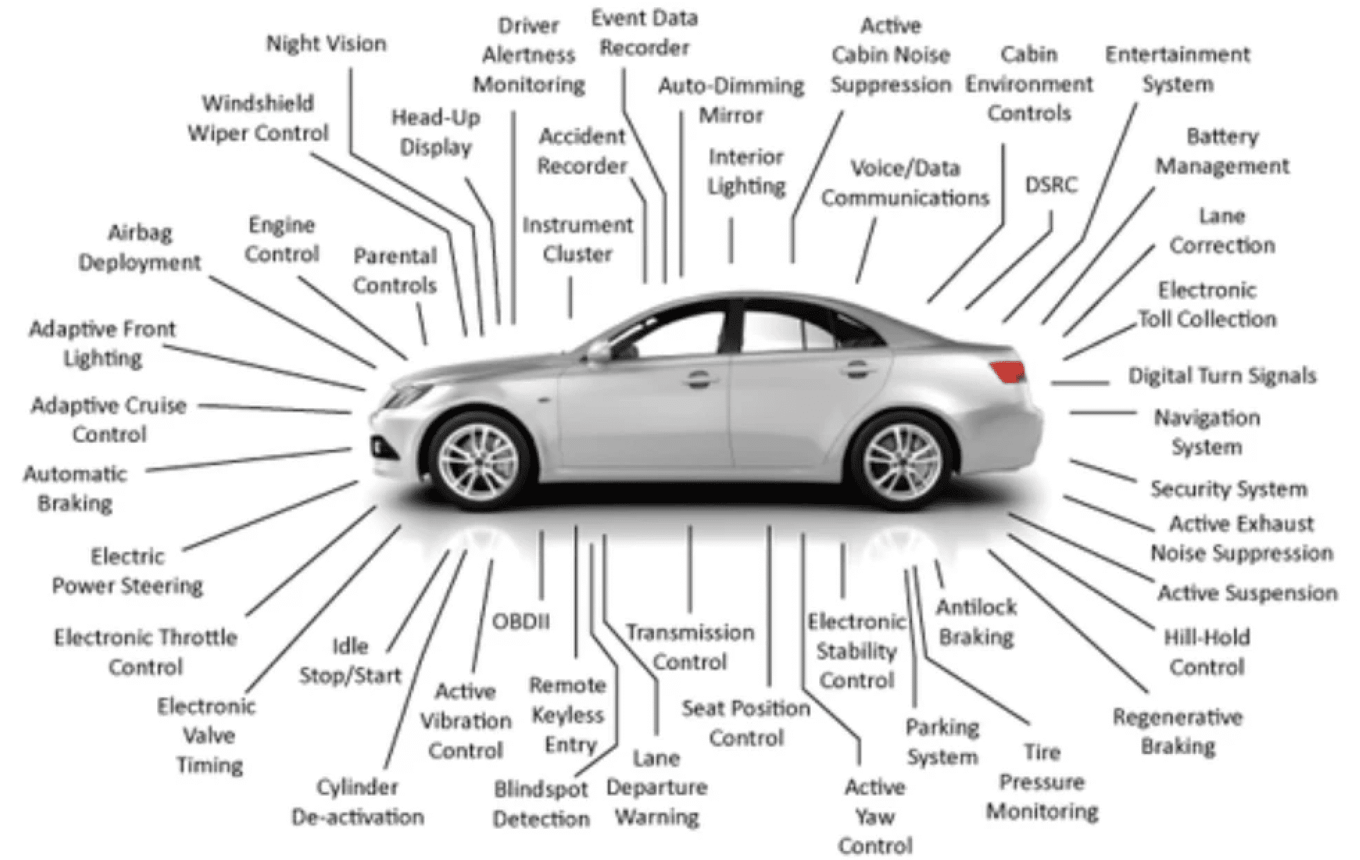
\includegraphics[width=0.9\textwidth]{images/vehicle_processors.png}  % Sostituisci 'nome_immagine' con il nome del tuo file immagine e l'estensione
  \caption{An incomplete overview of computers in a modern car \cite{ieeeSoftwareDefinedVehicle}}
  \label{fig:VheicleProcessors}
\end{figure}

This paradigm shift has been driven in part by the introduction of autonomous driving. To ensure maximum safety, a car must be equipped with dozens of sensors that can constantly collect data about what is happening to the vehicle and its surroundings. The number of these telemetry devices, which are nothing more than specialized IoT devices for the automotive world, also known as \gls{ac:tcu}, is expected to grow as autonomous driving technologies advance. In addition to data collection, another key issue is data analysis. Modern vehicles are caught between low-power systems for maximum vehicle efficiency and high-performance systems for analyzing the collected data and making excellent decisions in a short time.

However, the proliferation of processors within vehicles, orchestrating communication to manage diverse components, presents a formidable challenge; each component often integrates a processor with unique logics, diverging from the logics embedded in processors of other components. Complicating matters further, these components are frequently supplied by companies with proprietary management logics, not readily accessible to the automotive companies themselves.

In addressing this intricate scenario, the transformative concept of a \gls{ac:sdv} comes to the forefront. Defined as "any vehicle that manages its operations, adds functionality, and enables new features primarily or entirely through software"  \cite{blackberrySDV}, the notion of \gls{ac:sdv}, with all the associated technologies, offers a comprehensive solution to the challenges posed by the intricate interplay of software and hardware in modern vehicles.

One of the main benefits of this innovation in the automotive industry is the ability to have easily manageable systems. In the past, due to their high level of specialization for performance and low power consumption, automotive computer systems were developed and tested directly on the devices themselves, often in a manual way. This resulted in a large consumption of resources and a waste of time. Today, the goal is to have cloud infrastructures that ensure a more agile development and testing process due to the presence of general-purpose systems in the vehicle.

Consequently, the use of \gls{ac:sdv} aims to completely separate software and hardware, allowing the production of high-level software on entirely generalized hardware systems. This results in significant savings in terms of time and money for hardware production, along with providing an advantage in terms of security due to the simplification of software.

Another very important aspect of \gls{ac:sdv}, which will be analyzed in the following chapters, is that since a \gls{ac:sdv} is by definition characterized by the ability to dynamically and flexibly update software, this solution offers significant security advantages in several aspects:
\begin{enumerate}
  \item \textbf{Human Safety Critical Security:} From the moment that a vehicle can be classified as safety critical (as it is reported in the standard ISO 26262-1:2018 of the ISO society where is said that "safety is one of the key issues in the development of road vehicles" \cite{ISO26262}), the elimination of software vulnerabilities related to the vehicle's systems is crucial for the overall safety of the vehicle itself.  
  \item \textbf{Intrinsic Software Security:} This approach allows for the prevention and resolution of vulnerabilities unknown at the time of software design, contributing to ensuring a high standard of security. For example, as demonstrated by NIST in the research on the Analysis Of The Impact Of Software Complexity \cite{NISTCodeComplexity}, the increase in software complexity in different cases results in less analyzable programs. In some instances, the same vulnerability analysis tool may detect vulnerabilities, while in others, analyzing the same code, it may not. 
\end{enumerate}

Effectively navigating the development of \gls{ac:sdv} technology necessitates a collaborative approach across diverse companies, particularly in the realms of hardware and cloud computing. For this reason, many software, hardware, and automotive companies are involved in the development of this innovation, which aims to become a standard in vehicle production for the entire automotive industry.

In order to carry out the research and analysis of the new technologies described above, as well as to get involved in the practical side of things, it was essential to find a company that had both the IT skills needed to interface with cloud technologies and experience in the world of automotive manufacturing and software production. The partner company with which the practical design and implementation of the working explanatory example was carried out is introduced below.
\section{Partner Company}

Leveraging extensive experience in the cloud industry and fostering deep-rooted relationships within the automotive sector, Storm Reply stands out as the ideal choice to lead the project discussed in this thesis. A key player in the Reply group, Storm Reply specializes in designing and implementing innovative Cloud-based solutions and services \cite{StormReplySite}. 

With a broad client base spanning multiple sectors, particularly the automotive industry, the company's expertise played a pivotal role in fully understanding the project's context and internal dynamics. This extensive knowledge provided the cornerstone for the development of a tangible example of the infrastructure.

\begin{figure}[h]  % 'h' significa che la figura viene posizionata qui
  \centering
  
\includegraphics[width=0.3\textwidth]{images/Storm_Reply_logo.png}  % Sostituisci 'nome_immagine' con il nome del tuo file immagine e l'estensione
  \caption{Logo of the partenr company of the project}
  \label{fig:StormReplyLogo}
\end{figure}

Among the main customers in the automotive world of the consulting company, we can mention Ferrari, one of the most important companies in motor sports competitions and in the production of luxury cars, and Stellantis, one of the biggest giants in the automotive industry as well as in the global market. Although different, these two companies interact with Storm Reply to take advantage of its great knowledge in the cloud world and in the management of AWS services. Thanks to the connection with these important companies it was possible to receive essential information for the thesis work.

One great advantage of collaborating with this company is the wide availability of resources, both material and, above all, in terms of experience. As a large IT consultancy company, Reply is divided into many sub-business units, that makes possible the nteraction with various realities, ranging from embedded to low-level development, network and security infrastructure management, and web services management. Furthermore, there is a research and development section called Area 42 where entities can interact and influence each other to create innovative projects.

A point of pride for Storm Reply is its recognition as an Amazon Web Services (AWS) Premier Consulting Partner since 2014, ranking among the top Amazon Partners globally. This distinctive characteristic underscores the decision to develop the infrastructure using Amazon Web Services.

According to the official AWS description page \cite{AWSGlobalInfrastructure} the AWS Cloud spans 102 Availability Zones within 32 geographic Regions around the world and servs 245 countries and territories. With millions of active customers and tens of thousands of partners globally, AWS has the largest and most dynamic ecosystem. AWS is evaluated as a Leader in the 2022 Gartner Magic Quadrant for Cloud Infrastructure and Platform Services (a series of market research reports published by IT consulting firm Gartner that rely on proprietary qualitative data analysis methods to demonstrate market trends, such as direction, maturity and participants), placed highest in Ability to Execute axis of measurement among the top 8 vendors named in the report.

\begin{figure}[h]  % 'h' significa che la figura viene posizionata qui
  \centering
  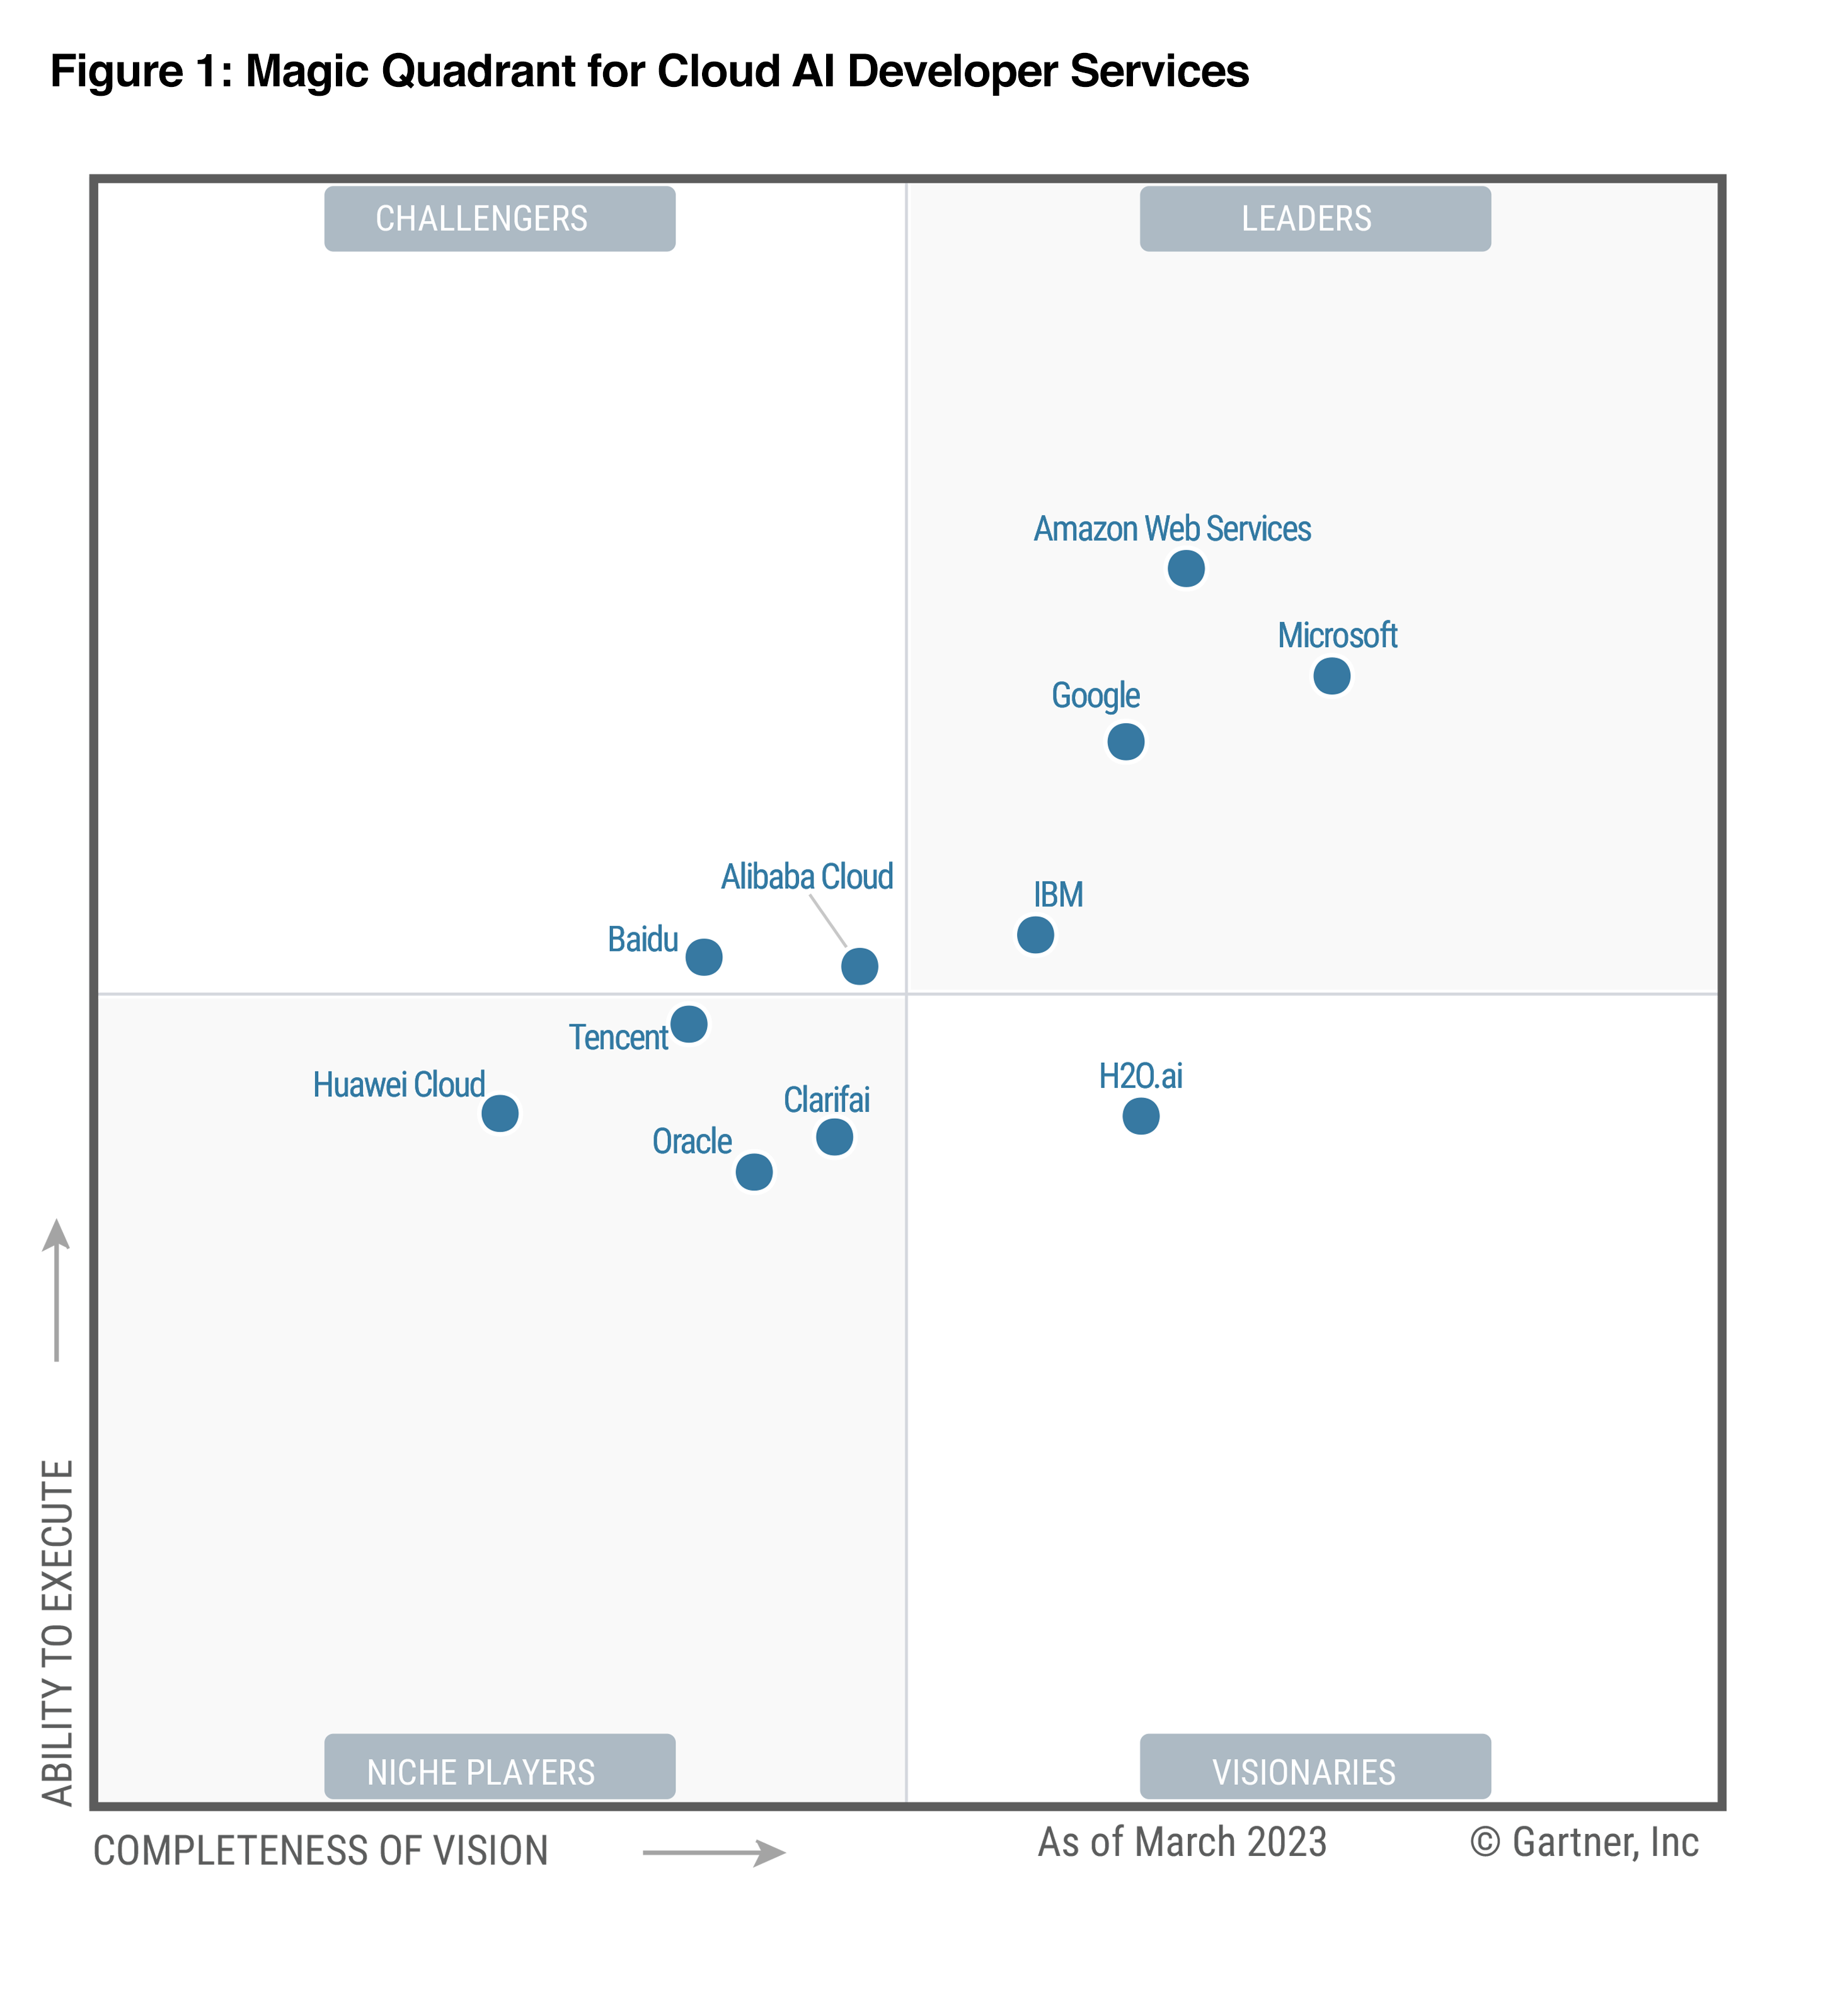
\includegraphics[width=0.6\textwidth]{images/AWSMagicQuadrantForCloud.png}  % Sostituisci 'nome_immagine' con il nome del tuo file immagine e l'estensione
  \caption{The Gartner Magic Quadrant for Cloud Infrastructure and Platform Services \cite{GartnerMagicQuadrant}}
  \label{fig:AWSMagicQuadrantForCloud}
\end{figure}

The infrastructure exhibits several key attributes contributing to its robustness and efficiency: 
\begin{itemize} 
  \item \textbf{Security:} The infrastructure undergoes 24/7 monitoring to ensure the confidentiality, integrity, and availability of data. All data flowing across the AWS global network is automatically encrypted at the physical layer before leaving secured facilities.
  \item \textbf{Availability:} To ensure high availability and isolate potential issues, applications can be partitioned across multiple AZs (Availability Zones) within the same region, creating fully isolated infrastructure partitions.
  \item \textbf{Performance:} AWS Regions offer low latency, low packet loss, and high overall network quality. This is achieved through a fully redundant 100 GbE fiber network backbone, often providing terabits of capacity between Regions.
  \item \textbf{Scalability:} The AWS Global Infrastructure allows companies to take advantage of the virtually infinite scalability of the cloud. This enables customers to provision resources based on actual needs, with the ability to instantly scale up or down according to business requirements.
  \item \textbf{Flexibility:} The AWS Global Infrastructure provides flexibility in choosing where and how workloads are run, whether globally, with single-digit millisecond latencies, or on-premises.
  \item \textbf{Global Footprint:} AWS boasts the largest global infrastructure footprint, continually expanding at a significant rate.
\end{itemize}
Thanks to its expertise and qualifications, Storm Reply is able to provide the above features to its customers, offering a comprehensive consultancy service for managing cloud infrastructures.

\section{Thesis Objective}
In the automotive context, the use of \gls{ac:sdv} plays a crucial role in terms of cost, innovation and safety. The objectives of the thesis are intertwined with the opportunities offered by \gls{ac:sdv} technology, for instance addressing the primary challenge of overcoming the current difficulties associated with the presence of different specialized hardware platforms on the same vehicle, to make the vehicle a more efficient and safer device based on software as a fundamental element.

One of the main objectives of this thesis is to propose the opportunity offered by \gls{ac:sdv} solution capable of eliminating various phases of the software production pipeline. This would result in significant time and cost savings, enabling the investment of these resources in other areas.

From a practical standpoint, the project's goal is to provide, through the use of AWS services, a cloud infrastructure capable of managing the \gls{ac:sdv} both in terms of software production and data analysis.

The work begins with an overview of the state of the art of software development in the automotive world, comparing the goals of the future with the techniques used in the past. For this purpose, the weaknesses of the sector are explained in order to highlight the advantages of \gls{ac:sdv} technology.Next, some definitions of the technologies that can bring the development of a paradigm shift in \gls{ac:sdv} benefits are provided. Finally, an example of an initiative proposed as a first attempt to standardize the \gls{ac:sdv} concept is presented, namely the SOAFEE project.

The work continues with an introduction to cloud computing, which is the programming approach that accompanied the entire project from beginning to end. The characteristics of this technique are analyzed, especially the advantages it can bring, and the example of how AWS manages to best enhance the potential of cloud computing is shown. Special attention is given to the security aspect, as it is a fundamental objective of the thesis topic, but also central element of the idea behind the cloud development of the AWS company and the project partner company.

Moving towards the description of the implementation of the practical project, it is possible to arrive at the exploration of the AWS services used. In order to make the realization of the project possible, as described several times throughout the thesis, it is necessary to rely on this type of service. With the aim of introducing the characteristics of the services used, an extensive descriptive list is provided.

The last part of the thesis deals with the actual implementation of the project, with the purpose of providing a concrete and working example of what has been described in the previous chapters. The implementation begins with the creation from scratch of a device capable of simulating telematic data, develops in the construction of a cloud infrastructure with the services mentioned above, and ends with the exploration of the tool used for data analysis.

Finally, to conclude the research, the results of the final presentation of the operation of the whole system on a real device are shown. In addition, a final evaluation of the whole project is made and the future possibilities opened by the work are shown.
\lstdefinestyle{mystyle}{
    backgroundcolor=\color{myyellow},
    basicstyle=\ttfamily\small,
    breaklines=true,
    frame=single,
    language=XML
}

\chapter{State-of-the-Art Analysis} \label{ch:state-of-the-ArtAnalysis}
The following chapter constitutes an in-depth exploration of current technologies and methodologies within the automotive industry, with a specific focus on the complexity of vehicular software development. Firstly, the current automotive landscape will be examined, providing a detailed insight into challenges associated with software development in vehicles.

Subsequently, through meticulous analysis of scientific publications, technical reports, and practical implementations, the chapter delves into the radical transformation of the automotive sector facilitated by the concept of Software Defined Vehicle (SDV). This technology, crucial for technological progress and vehicular safety, will be explored from various perspectives. Particularly, the synergy between Cloud, software, and hardware will be investigated, highlighting solutions proposed by major industry players and analyzing their applications, benefits, and limitations.

The objective is to offer a comprehensive overview of current dynamics, emphasizing the pivotal role of SDV in the evolution of the automotive industry.

\section{Current Automotive Software Development}

In the past, the automotive industry advanced primarily through the development of technologies in mechanical engineering, focusing on perfecting combustion engines. Nowadays, the paradigm has radically changed due to multiple factors, including electrification, automation, shared mobility, and connected mobility.

Software technology development in the automotive field can be metaphorically compared to what has happened in smartphone development, as highlighted in the manifesto document regarding Bosch's Software Defined Vehicle (SDV) \cite{SDVBoschMobility}.

The ultimate goal is to achieve simple and user-friendly devices that fully meet the user's needs. Currently, many customers express dissatisfaction because their cars do not offer the same functionality and ease of use common in smartphones. Many ask: Why can't my \$50,000 car perform the same tasks as my \$300 smartphone?

A key difference between the automotive and smartphone industries is the level of complexity, which brings with it a number of issues.

\subsection{difficulties}
We can analyse in depth the problems of the current automotive software that is being developed via 4 main difficulties:

\begin{itemize}
    \item \textbf{Specialized Hardware:} Today's vehicles are still complex systems of systems. Each subsystem in a car, from brakes to transmission, is a complex entity, supplied by a different manufacturer and integrated with a unique software architecture. The level of complexity and the need for seamless interoperability between systems far exceeds that of today's smartphones.
    \item \textbf{Time:} The software production pipeline involves many development and testing steps with a not inconsiderable amount of time spent on each one. This is greatly increased by the presence of different components, so development time must be considered for each different unit of the system.
    \item \textbf{Cost:} The complexity of the software systems in vehicles entails very high costs, aggravated by the fact that the test phase is often carried out directly on the boards (for hardware requirements), which means a much longer production process, especially in the event of errors.
    
    \begin{figure}[h]  % 'h' significa che la figura viene posizionata qui
        \centering
        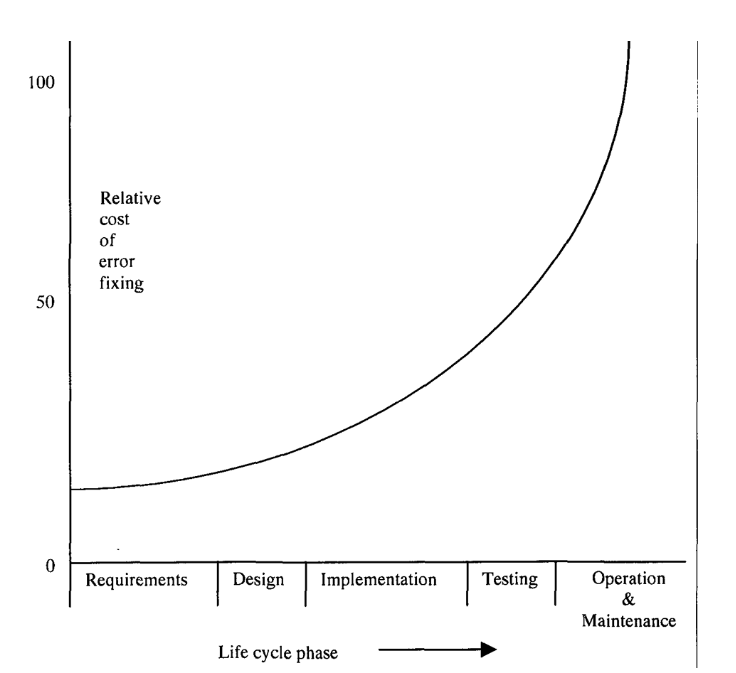
\includegraphics[width=0.9\textwidth]{images/costs_of_errors_correction_in_software_development.png}  % Sostituisci 'nome_immagine' con il nome del tuo file immagine e l'estensione
        \caption{Cost of fixing errors increases in later phases of the life cycle \cite{CostsOfSoftwareDeveloping}}
        \label{fig:CostsOfSoftwareDeveloping}
      \end{figure}

    \item \textbf{Human Safety Security:} Automotive embedded software must meet stringent reliability and security requirements, while delivering performance and a reasonable memory footprint. To develop automotive embedded software, you need the right tools that meet safety and security standards to evaluate, prototype and test your software.
\end{itemize}

What lessons can be drawn from the study of barriers that can be applied to the vehicle lifecycle? Historically, the vehicle lifecycle has been characterised by the simultaneous production and deployment of tightly integrated hardware and software. Once the vehicle was in the hands of the consumer, its characteristics remained largely unchanged until the end of its life. However, the SDV paradigm introduces the possibility of decoupling hardware and software release dates, a prerequisite for adopting a digital-first approach. This approach brings the design and virtual validation of the digital vehicle experience to the forefront of the lifecycle.
It also requires the application of the digital-first concept, which means that new ideas for the vehicle experience are first explored in virtual environments to ensure early user feedback, long before any custom hardware needs to be developed or a physical test vehicle is available. Digital first is the application of design thinking and lean startup principles, originally rooted in internet culture, to the tangible realm of automotive development.

%“Automakers and their suppliers need to continuously review and improve the testing approach in design and development, as well as look for new tools that automate and increase test coverage of their products,” Giallorenzo explained. “Cloud emulation is a major innovation that is coming to the industry to facilitate development and testing. Historically, testing of embedded software solutions has been hindered by the lack of chipsets and hardware, which is required to properly test complete hardware-plus-software solutions. This was particularly painful during the recent COVID-induced supply chain crunch."

\section{Introduction to Software Defined Vehicle}
The Software Defined Vehicle represents the new frontier of automotive manufacturing and is poised to completely change the paradigm of automotive production. 

If we imagine bringing a feature update to one of today's vehicles, it will most likely take anywhere from one to seven years from the idea to when that feature is actually perceptible in the production vehicle; this takes so long because the vehicles produced up to this point have not been designed with frequent updates in mind \cite{SDVBosch}.
Traditionally focused on physical functionality, the automotive industry has evolved from early electronic features such as airbags, vehicle stabilisation and braking systems to modern driver assistance and even automated driving. 
The current shift towards a digital experience is possible thanks to vehicle design that includes software integration as a fundamental part. Software should no longer be seen as an accessory to the vehicle, but as an integral part of the vehicle itself.

The simultaneous efforts of major automotive companies such as Bosch, Renault and Stellantis, in collaboration with leading computer developers such as Arm, BlackBerry and AWS, have given rise to the Software Defined Vehicle concept, which they define as "any vehicle that manages its own operations, adds functionality and enables new features primarily or entirely through software" \cite{blackberrySDV}.

The Software Defined Vehicle solution is nowadays being considered by several companies as the manifesto of a new era of vehicle development. An example is given by the Renault Group, which in an overview of its products describes: "Today, it is already possible to make remote updates of some vehicles via the Firmware Over The Air (FOTA) system. This keeps the vehicle safe by making it easier and faster to improve the on-board system and apply patches. Tomorrow, the Software Defined Vehicle's flexible and scalable architecture will enable the faster development and integration of new features throughout the vehicle lifecycle, directly into the cloud, that is, in secure online servers accessible from anywhere and anytime" \cite{SDVRenault}. 

It is evident that Software Defined Vehicles represent the future of the automotive industry, promising an enriched and sustainable user experience as vehicle technologies evolve. This section further clarifies the current state of the industry, highlighting the key enablers that are allowing the development of the SDV paradigm and the benefits of this innovation.

\subsection{Enablers}

There are mainly three fundamental technologies that contribute to the realisation of the Software Defined Vehicle: standardized hardware, cloud and over-the-air (OTA) updates via OTA servers, all developed by leading companies in the computing industry. In this section, each technology will be analysed with reference to concrete examples from the current market.

\begin{itemize}
    \item \textbf{Standardized hardware} 
    
    One of the most important aspects of Software Defined Vehicle is the separation of software from hardware. To achieve this, it is essential to move away from the approach of using dedicated hardware for each vehicle component system, and instead favour an approach based on general purpose processors that are as centralised as possible. This transition not only promotes ease of software development and scalability, but also offers the opportunity to create parity between the virtual development and test environment and the real execution environment.
    
    Several players in the semiconductor industry have stepped up to the challenge of realising this vision, including Arm. Through the development of energy-efficient processors, Arm is present in every part of the vehicle, from high-performance systems in advanced driver assistance systems (ADAS), automated driving (AD), in-vehicle infotainment (IVI) and digital cockpits, to gateway, body and microcontroller endpoints \cite{ArmAutomotive}. The aim is to create Arm-based MCUs that enable implementation of a common architecture, scalability between applications to meet processing requirements, software reuse and reduced development costs.
    
    Another major player is Qualcomm, which is being adopted by the Renault Group through its Snapdragon Digital Chassis vehicle architecture, a set of cloud-connected platforms for telematics and connectivity, digital cockpits, assistance and driver autonomy.

    \item \textbf{Cloud} 
    
    Using a cloud platform that offers scalable and secure solutions for real-time application updates, increased connectivity and efficient data management is essential for SDV. 

    Well-known companies such as Amazon Web Services (AWS) and Google Cloud are already present in the automotive industry as partners of partner of many automotive companies. The AWS services and technologies will be in depth described in the futher chapters.
 
    \item \textbf{Over-The-Air updates}
    
    An Over-The-Air (OTA) update is the remote and wireless transfer of applications, services, firmware and configurations from a server to a target device. This process takes place over an available network, preferably the Internet. The main purposes of OTA are to remotely update software or firmware, provide power-safe procedures to ensure that the device will boot even if power is lost during the update process, maintain a robust implementation, ensure data protection and reduce overall maintenance costs \cite{Open-sourceSWUpdate}.

    In the context of the thesis, it is crucial to acknowledge that the implementation of OTA updates may increase the vulnerability of automotive systems to hacking and other cyber attacks. These vulnerabilities could potentially be exploited by hackers to gain unauthorised access to private information, take remote control of the vehicle or even cause it to malfunction. Another significant issue is the leakage of information about updates and their sources. This can enable malicious actors to introduce viruses and malware, further exacerbating the security risks associated with OTA updates \cite{EnhancedMulti-LevelSecureUpdate}. 
    
    To perform an OTA update, both a client on the vehicle, responsible for waiting and checking for incoming updates, and a server, facilitating the availability of the update broadcast to all connected devices, are essential. In this context, Autosar can be considered, as it represents a standard and open source architecture for intelligent mobility \cite{AutosarAbout}, which includes a dedicated platform for client and server management of OTA updates. Another notable example is Hawkbit, which serves as a backend framework for deploying software updates to edge devices and is being developed by the Eclipse Foundation; this tool will be discussed in more detail in later chapters as it will be used to create a proof of concept. The final tool of note is AWS Greengrass, an edge agent manager for managing software updates in edge IoT devices, provided by AWS; this tool will also be discussed in later chapters as an alternative solution to the client manager.
    
    \item \textbf{MQTT communication}
    
    The Message Queuing Telemetry Transport (MQTT) is a standardized protocol, specified by ISO/IEC 20922:2016 and developed by the Oaesis organization. It enables the exchange of Application Messages over a network connection, providing an ordered, lossless stream of bytes from the Client to Server and Server to Client without the need to support of a specific transport protocol.

    In an MQTT transport, an Application Message carries payload data, a Quality of Service (QoS), a collection of Properties, and a Topic Name. Clients, which can be programs or devices, perform various actions such as opening and closing network connections, publishing Application Messages, subscribing to requested Application Messages, and managing subscriptions \cite{MQTTVersion5.0}.

    On the Server side, it acts as an intermediary between publishing and subscribing Clients. The Server accepts network connections, processes Subscribe and Unsubscribe requests, and forwards Application Messages matching Client Subscriptions. The Server, also known as the Broker, essentially coordinates messages among various Clients. Its responsibilities extend to authorizing and authenticating MQTT Clients, transmitting messages to other systems for further analysis, and managing tasks such as handling missed messages and Client sessions \cite{MQTTAWS}.

    Sessions, representing stateful interactions between Clients and Servers, can last for the duration of a Network Connection or span multiple consecutive connections.
     \begin{figure}[h]  % 'h' significa che la figura viene posizionata qui
        \centering
        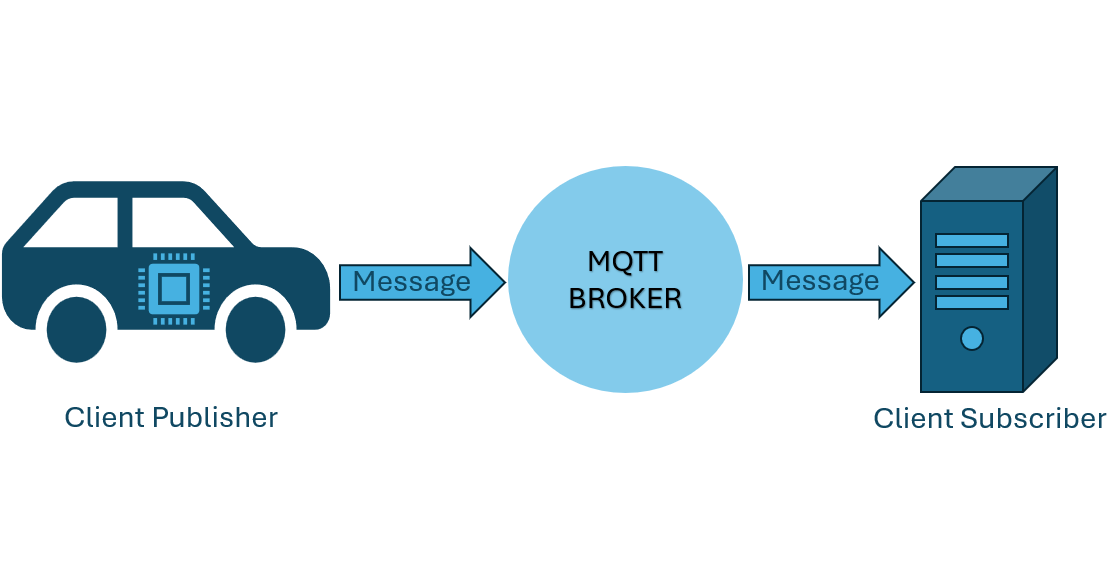
\includegraphics[width=0.8\textwidth]{images/MQTTProtocol.png}  % Sostituisci 'nome_immagine' con il nome del tuo file immagine e l'estensione
        \caption{A simple representation of communication using the MQTT protocol}
        \label{fig:MQTTProtocol}
    \end{figure}

    The MQTT protocol can be used in SDV, both for sending data produced by the vehicle to the cloud servers and for sending updates from the servers to the vehicle. This is because the MQTT protocol allows asynchronous and misaligned communication even in the presence of poor connectivity, a situation that cannot be underestimated in the automotive field.
\end{itemize}

The collaborative efforts of this technologies contribute to advancement of SDV for makeing vehicles not only defined by their physical attributes but also as dynamic entities that can be continuously updated through software.

\subsection{Benefits}
The Software Defined Vehicle, as introduced in the previous chapters, brings several benefits to both automotive companies and the end-user experience.  These innovations are made possible by the fact that the vehicle becomes a device that can be constantly monitored and updated in real time via the cloud throughout its entire lifecycle. Let us now look at the key benefits.

From the point of view of this project, the main innovation brought by this technology is the security of the device software. Since, as mentioned above \cite{ISO26262}, vehicles are considered as safety elements critical to human life, the safety benefits can be analysed from two perspectives:
\begin{itemize}
    \item \textbf{Human Safety Critical Security:} The ability of SDV to receive real-time data from the vehicle allows in-depth monitoring of all its components. Taking the influence of tyres as an example, it has been found that most road accidents are caused by tyre wear and lack of regular maintenance. It is therefore necessary to assess the health of tyres through continuous monitoring of physical parameters such as tyre thickness, temperature and pressure, as well as regular maintenance. This helps to eliminate or minimise the possibility of tyre bursts and subsequent accidents. It also improves the safety of people and vehicles \cite{PredictDefectsOfTiresInHeavyVehicle}. These factors can be monitored either manually or automatically: manual predictive maintenance requires human intervention and can lead to some errors; automatic predictive maintenance using artificial intelligence can be more efficient \cite{AirPressureSystemFailurePrediction}. Renault defines this work as "predictive maintenance" \cite{SDVRenault}, stressing the importance of collecting and analysing data in a centralised system to anticipate and prevent potential failures, ensure the safety of people, reduce maintenance costs and improve the performance of the vehicle.
    \item \textbf{Intrinsic Software Security:} In the presence of bugs and vulnerabilities in the vehicle's software, SDV makes it possible to intervene promptly to resolve each problem and reduce the window of exposure.
    \begin{figure}[h]  % 'h' significa che la figura viene posizionata qui
        \centering
        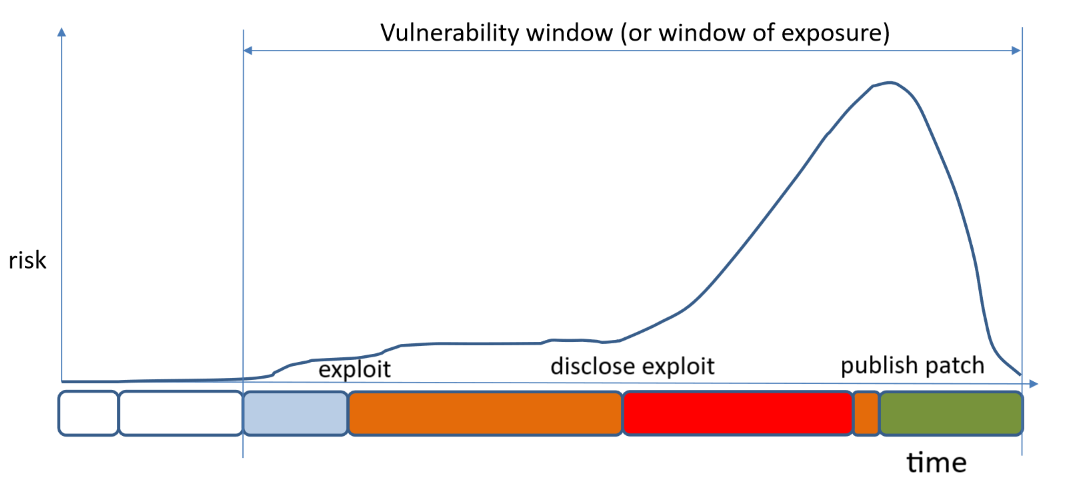
\includegraphics[width=0.8\textwidth]{images/window_of_exposure.png}  % Sostituisci 'nome_immagine' con il nome del tuo file immagine e l'estensione
        \caption{Risks and time relationship in the various phases of a vulnerability lifecycle}
        \label{fig:WindowOfExposure}
    \end{figure}

    A crucial aspect of vehicle software security is the robustness of the algorithms, especially in the context of autonomous driving. In this context, a predictive algorithm responsible for vehicle safety decisions can be continuously improved and optimised. The SDV also introduces the concept of the 'digital twin', a platform that virtually replicates the functionality and behaviour of the vehicle. Thanks to this technology, predictive algorithms used in autonomous driving can be effectively tested on the cloud platform and, when ready, integrated directly into the vehicle.
\end{itemize}

From a user experience point of view, two other significant benefits can be identified: an increase in the value of the vehicle, which can be continuously upgraded over time, and the ability to enable additional vehicle functions via software. For example, the user can decide to activate a feature for a certain period of time and then deactivate it (paying only for the time it is used), or activate a new feature that was not available at the time of purchase. In essence, the vehicle becomes a dynamic platform that is constantly evolving and fully customisable through the software.

For automotive companies, the benefits mentioned so far can bring direct benefits to the industry. In support of this, Stellantis reports that: "the team in Poland will contribute to the global software creation network that is key to Stellantis' work in creating software-defined vehicles (SDVs) that offer customer-focused features throughout the vehicle's life span, including updates and features that will be added years after the vehicle is manufactured. “Creating an infrastructure inside our vehicles that easily and seamlessly adapts to meet driver expectations is a key element of Stellantis' global drive to deliver cutting edge mobility. Stellantis' software-driven strategy deploys next-generation tech platforms, building on existing connected vehicle capabilities to transform how customers interact with their vehicles and to generate €20 billion in incremental annual revenues by 2030".

In addition, the SDV paradigm brings an advantage from a software production pipeline perspective. In today's software production scenario, there can be two development mechanisms:
\begin{itemize}
    \item A more traditional mode in which software is created directly on the system, hence on the processor itself. This is undoubtedly the most inconvenient solution, as it would require unnecessary overuse of processors, wasting resources, money and time.
    \item Alternatively, developers rely on cumbersome operating system emulation tools on the host machine and the cross-compilation process, which uses a dedicated compiler to produce executable code for the target system. Once the code is on the development system, a final integration and validation test can be performed, but scalability is limited to the number of physical hardware platforms. 
\end{itemize}

Typical workflows for the development, integration and validation of embedded systems are as follows \cite{DevelopersWorkflow}:
\begin{figure}[h]  % 'h' significa che la figura viene posizionata qui
    \centering
    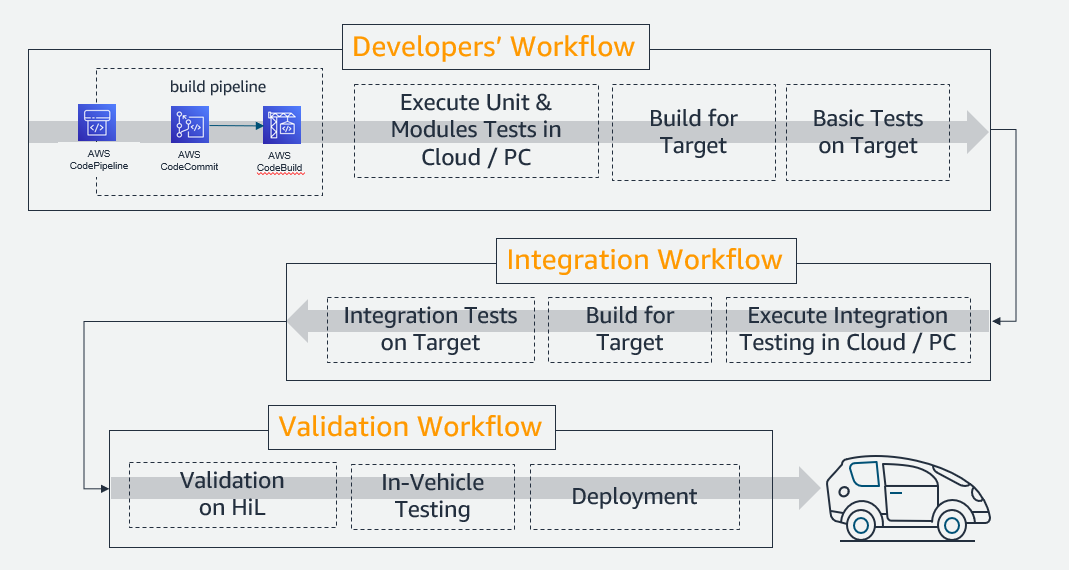
\includegraphics[width=0.7\textwidth]{images/today_developer_workflow.png}  % Sostituisci 'nome_immagine' con il nome del tuo file immagine e l'estensione
    \caption{today development, integration, and validation workflows for embedded systems}
    \label{fig:TodayDeveloperWorkflow}
\end{figure}

As explained in the following chapters, by using the software defined vehicle, i.e. operating systems that rely on general purpose porpouse architectures to provide parity between cloud and edge systems, it is possible to reduce the embedded developer's workflow to remove many of the steps that are now no longer required, as shown in the diagram below \cite{DevelopersWorkflow}:
\begin{figure}[h]  % 'h' significa che la figura viene posizionata qui
    \centering
    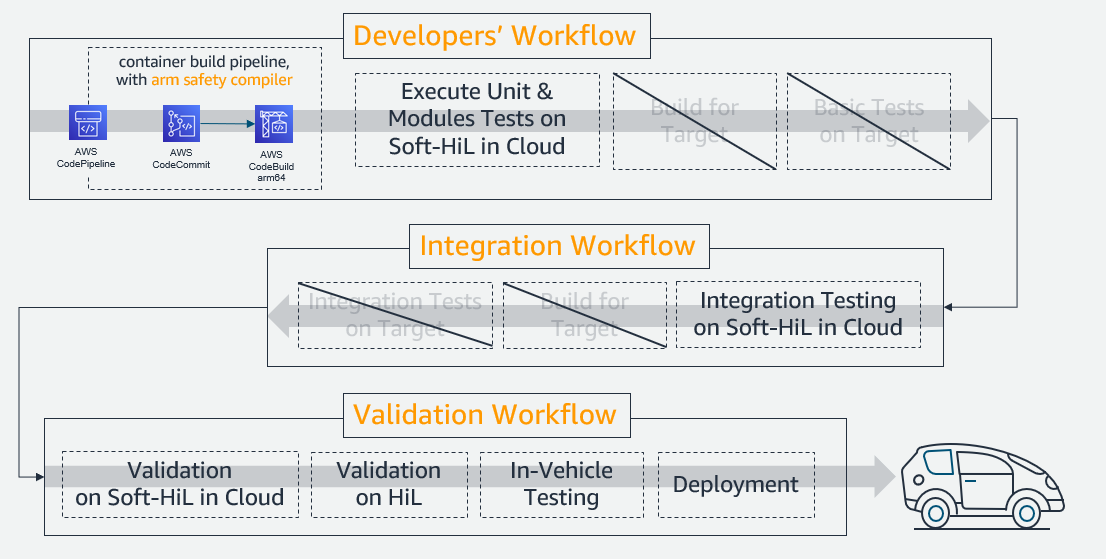
\includegraphics[width=0.7\textwidth]{images/future_developers_workflow.png}  % Sostituisci 'nome_immagine' con il nome del tuo file immagine e l'estensione
    \caption{future development, integration, and validation workflows for embedded systems}
    \label{fig:FutureDevelopersWorkflow}
\end{figure}

\subsection{initiatives: SOAFEE}
In 2021 Arm, AWS, and other founding members announced the Scalable Open Architecture for Embedded Edge (SOAFEE) Special Interest Group, which brings together automakers, semiconductor, and cloud technology leaders to define a new open-standards based architecture to implement the lowest levels of a software-defined vehicle stack. \cite{DevelopersWorkflow}

SOAFE is created to achive Software Defined Vehicle, and for doing that four-pillar principle are used \cite{SoafeeProject}:
\begin{enumerate}
    \item Standards: standardization ensures interoperability and compatibility among various software components, fostering a cohesive ecosystem for Software Defined Vehicles.
    \item New software architecture and methodologies: this involves transitioning from traditional monolithic architectures to more modular and scalable designs; the incorporation of agile development practices and DevOps methodologies ensures efficient and continuous software evolution.
    \item Industry collaboration: Fostering partnerships, knowledge sharing and collaboration among key stakeholders, including automakers, technology companies and regulators, is essential.
    \item Vehicle simulation: simulated environments allow in-depth testing and refinement of software functionality to ensure optimal performance and security under a variety of conditions.
\end{enumerate}
SOAFEE aims to adopt and enhance current standards used in today's cloud-native world to help manage the software and hardware complexity of the automotive Software Defined Vehicle architecture.

The core principles of safety, security, and real time are inherent in each pillar. It is fully expected that the SOAFEE architecture will support use-cases that execute safety-critical services alongside non-safety-critical ones. It is fully expected that the SOAFEE architecture will support use cases that execute safety-critical services alongside non-safety-critical services. As it is not reasonable to develop the whole platform according to one safety standard, the strategy is to develop only safety-critical elements according to ISO 26262 and to isolate them from the non-safety-critical elements in order to ensure spatial, temporal and communication isolation. All implementations pass security checks and follow a set of best practices /cite{SoafeeArchitectureOverview}.

The SOAFEE paradigm is based on a very sophisticated architecture becouse it should work in the same way in the vehicle and in the cloud and follow cloud native technologies while considering the automotive specific needs for safety and limited resource footprints \cite{SoafeeArchitecture}.
\begin{figure}[h]  % 'h' significa che la figura viene posizionata qui
    \centering
    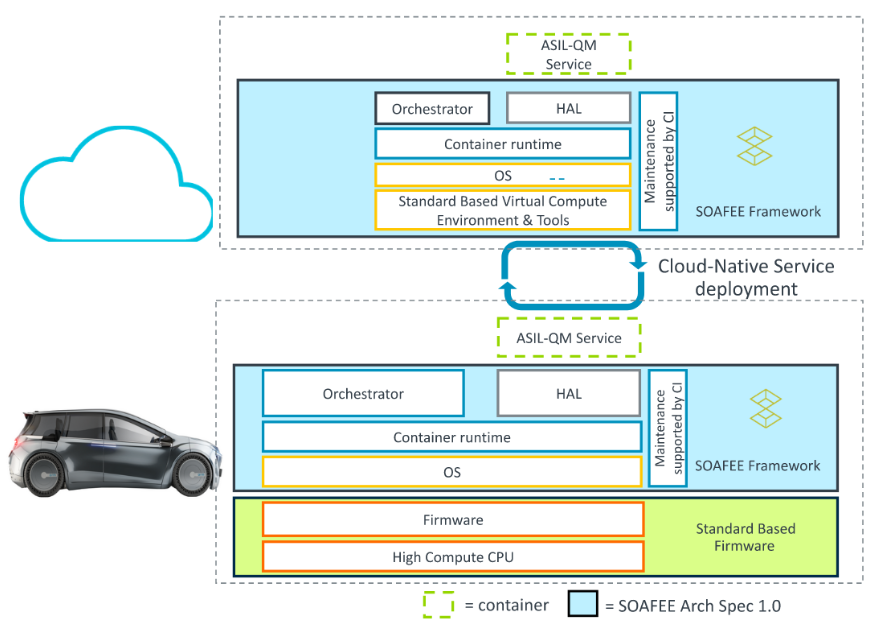
\includegraphics[width=0.7\textwidth]{images/SOAFEE_architecture.png}  % Sostituisci 'nome_immagine' con il nome del tuo file immagine e l'estensione
    \caption{SOAFEE Architecture v1.0 \cite{SoafeeArchitecture}}
    \label{fig:SoafeeArchitecture}
\end{figure}
%

\lstdefinestyle{yaml}{
     basicstyle=\color{red}\footnotesize,
     rulecolor=\color{black},
     string=[s]{'}{'},
     stringstyle=\color{red},
     comment=[l]{:},
     commentstyle=\color{black},
     morecomment=[l]{-}
 }
\chapter{Ideal Project Implementation} \label{ch:IdealProjectImplementation}


Negli ultimi anni numerose aziende che forniscono servizi agli utenti si sono trovate in serie difficoltà a causa dell' aumento sempre costante del numero
dei propri utenti e delle richieste di questi ultimi. Tali aziende si sono trovate quindi nella posizione di dover incrementare proporzionalmente le loro risorse disponibili, sia hardware che software, e di dover
assumere sempre più frequentemente del personale altamente specializzato per gestirle. Questa situazione di crisi ha portato ad un cambio di prospettiva in ambito aziendale, orientando l'attenzione verso un sistema di virtualizzazione
basato sull'utilizzo dei container invece che con le classiche macchine virtuali. Così facendo si è trovata una valida soluzione a questo problema, in quanto grazie alle loro caratteristiche i container consentono di garantire
la qualità del servizio offerto dalle aziende, ottimizzando l'utilizzo delle risorse hardware già in uso, senza la necessità di effettuare ulteriori investimenti significativi in hardware o personale aggiuntivo.\\
L'obiettivo di questo capitolo è di fornire una descrizione approfondita di una delle tecnologie più diffuse ed utilizzate in questo ambito, Docker\cite{docker-docs}. Inoltre viene anche descritto l'utilizzo di uno strumento, docker-compose, molto utile per 
creare e gestire applicazioni multi-container. Nella parte finale del capitolo è infine possibile trovare una descrizione e degli esempi su come eseguire il networking all'interno dei container.

\section{Differenze fra Container e Macchine Virtuali} 

Prima di scendere nello specifico descrivendo il funzionamento di docker all'interno di un sistema operativo è necessario definire nel dettaglio cosa sia una macchina virtuale e cosa un container e perchè è più efficiente la seconda soluzione rispetto alla prima.\\
Per quanto riguarda le macchine virtuali una definizione ci viene fornita dal sito ufficiale di VMware \cite{vmware}:\\
"Una Macchina Virtuale (VM) è una risorsa di elaborazione che utilizza software al posto di un computer fisico per eseguire programmi e distribuire applicazioni. Una o più macchine virtuali (guest) vengono eseguite su una macchina fisica (host). 
Ogni macchina virtuale esegue il proprio sistema operativo e funziona in modo separato dalle altre VM, anche quando sono tutte in esecuzione sulla stessa macchina host. Ciò significa che, ad esempio, una macchina virtuale con sistema operativo MacOS può essere eseguita su un PC fisico."\\

Sotto la prospettiva dei container, è possibile ottenere una definizione precisa consultando la documentazione ufficiale di Docker\cite{docker-container}.\\
"Un container è  un'unità standard di software che raggruppa il codice e tutte le sue dipendenze in modo che l'applicazione possa essere eseguita rapidamente e in modo affidabile da un ambiente di calcolo all'altro."\\

Seppur le due definizioni possano sembrare molto simili, la struttura software che sta dietro ad entrambe le tecniche di virtualizzazione è diversa, come viene mostrato nella seguente figura:\\


\begin{figure}[h]  % 'h' significa che la figura viene posizionata qui
    \centering
    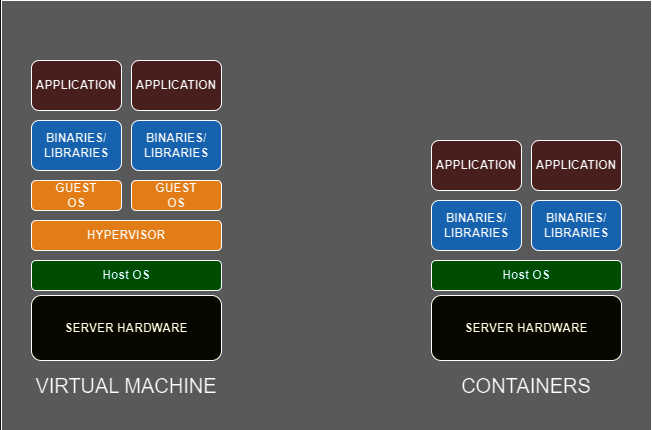
\includegraphics[width=1\textwidth]{images/VMvsContainers.png}  % Sostituisci 'nome_immagine' con il nome del tuo file immagine e l'estensione
    \caption{Architettura Virtual Machine e Containers}
    \label{fig:VMvsContainers}
\end{figure}
 
Le macchine virtuali hanno infatti una struttura più complessa rispetto ai container. È infatti presente un hypervisor\cite{hypervisor}, che è un software che permette di creare e gestire le macchine virtuali in maniera veloce, efficiente, flessibile e portabile.
Sopra all'hypervisor ogni macchina virtuale ha il suo proprio sistema operativo, costringendo l'host OS ad allocare numerose risorse per istanziare anche solo 1 macchina virtuale. Si può notare come questa soluzione sia difficlmente scalabile perchè
ciò porta il server hardware sul quale poggia tutto il sistema ad essere ulteriormente stressato con l'aggiunta di ogni macchina virtuale. Viceversa, i container richiedono solo le risorse minime necessaria a fare funzionare l'applicazione di turno, installando solo i file binari e le librerie necessarie.\\
Più in generale le caratteristiche vantaggiose dei container rispetto alle macchine virtuali sono riassunte dalle seguenti parole chiave:\\


\begin{itemize}
    \item \textbf{Modularità}: avere la possibilità di creare un container per ogni possibile task permette di suddividere i container in vari moduli, ognuno che svolge una sepcifica funzione del progetto di riferimento. Operando in tale direzione, è possibile sviluppare progetti con un approccio Bottom-Up
        , portando ad un ambiente di testing e validation più veloce ed immediato sui singoli moduli.
    \item \textbf{Isolamento}: ogni container che esegue una immagine viene visto come un ambiente isolato, indipendente dagli altri container in esecuzione. Questo approccio semplifica notevolmente l'individuazione di possibili bug ed errori nel progetto.
    \item \textbf{Peso in Memoria}: come analizzato nel lavoro di Martin Lindström\cite{performance-container}, differentemente dalle macchine virtuali, i container sono delle virtualizzazioni molto più leggere e che richiedono meno risorse alla macchina ospitante. Questo è derivato dal fatto che i container contengono solo lo stretto necessario all'applicazione per funzionare correttamente,
        mentre le VM hanno bisogno anche di istanziare un proprio sistema operativo, che richiede una discreta quantità di spazio.
    \item \textbf{Scalabilità}: Avendo un peso molto ridotto rispetto alle macchine virtuali, la necessità di aumentare le performance e le dimensioni di un progetto trova nei container un ottimo fattore di scalabilità. È  infatti possibile scalare i sistemi sia verticalmente, perchè all'aumentare delle risorse del sistema operativo ospitante corrisponde un aumento della velocità di reazione dei container
    che orizzontalmente, perchè aggiungere una feature corrisponde nell'aggiungere un container al sistema già funzionante. 
    \item \textbf{Condivisone Risorse}: Attraverso i file di configurazione dei container è possibile condividere file con il container, che nell'ambiente isolato verranno considerate come risorse dedicate, anche se in realtà sono condivise. Ciò estende questa funzionalità se si mettono in comune le stesse risorse per più container. In questo caso sulle risorse verrà messo un lock che bloccherà le risorse fino a che
        uno dei container non abbia finito di utilizzarle, rilasciandole.
    \item \textbf{Fast Boot}:Non dovendo dipendere da nessun sistema operativo, i container possono avviarsi ed essere operativi molto più velocemente rispetto alle macchine virtuali.
    \item \textbf{Operazioni su disco}: Avendo un collegamento diretto con il sistema operativo le operazioni su  disco (scrittura, lettura e cancellazione) sono più veloci, portando ad un aumento delle performance per processi parallelizzabili.
\end{itemize}

\newpage

\section{Docker e la sua architettura}

Tra le piattaforme software disponibili per istanziare e gestire containers per applicazioni Docker riveste il ruolo di software leader nel settore.
Nato nel 2013 e progettato da Solomon Hykes nell'azienda dotCloud, Docker è un progetto open source. La differenza fondamentale dagli altri software è che
basa la maggior parte delle operazioni eseguibili su un demone chiamato appunto Docker, che svolge le operazioni di istanziazione dei container e la loro gestione.
Al fine di garantire ciò, il demone richiede come file di input delle \textit{"Immagini"}. Come è descritto nella documentazione di Docker\cite{docker-container}: 
"Un'immagine di container Docker è un pacchetto leggero, autonomo ed eseguibile di software che include tutto il necessario per eseguire un'applicazione: codice, runtime, strumenti di sistema, librerie di sistema e impostazioni."\\

L'architettura di Docker sfrutta il meccanismo client-server, della quale viene mostrata una rappresentazione:\\

\begin{figure}[h]  % 'h' significa che la figura viene posizionata qui
    \centering
    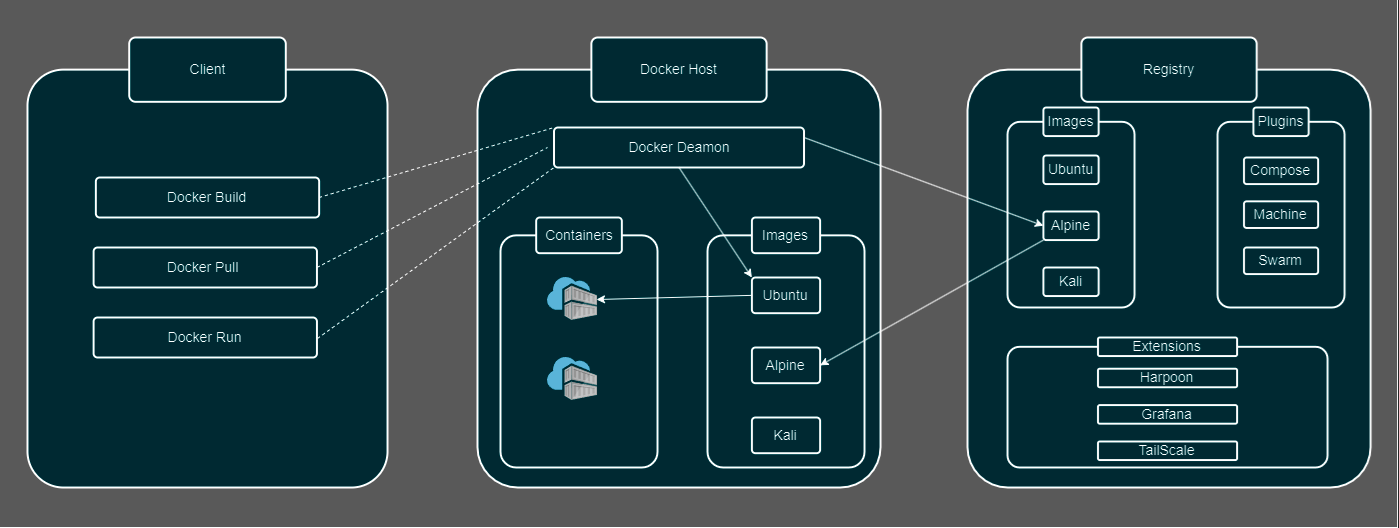
\includegraphics[width=1\textwidth]{images/Docker_Architecture.png}  % Sostituisci 'nome_immagine' con il nome del tuo file immagine e l'estensione
    \caption{Architettura Docker}
    \label{fig:DockerArchitecture}
\end{figure}

Di seguito una spiegazione di tutti gli elementi che intervengono nella creazione di un container:

\begin{itemize}
    \item \textbf{Docker Client}: Rappresenta la macchina fisica nel quale è installato Docker. Può comunicare con il controller principale (Docker Host) tramite delle Rest API.
    Le chiamate che il client può effettuare sono le seguenti:
        \begin{itemize}
            \item \textit{Docker Pull}: viene utilizzato per scaricare un'immagine da un Registro. Il demone controllerà se questa immagine è presente nel registro locale indicato, altrimenti andrà a cercare online
                la versione più recente dal registro predefinito di Docker Hub.
            \item \textit{Docker Build}: questo comando permette la creazione di un'immagine dato un file di configurazione definito dall utente (deve avere il nome di Dockerfile) e una cartella di riferimento.
            \item \textit{Docker Run}: questa chiamata fa creare al demone un container con l'immagine specificata da linea di comando ed avvia il container.
        \end{itemize}
    \item \textbf{Docker Deamon}: è il cuore dell'architettura di Docker. Il ruolo del docker deamon(anche chiamato dockerd) è di ascoltare le richieste tramite call API del client e gestire il registro Docker dove sono contenute
        le immagini, i plugin e le estensioni. Inoltre può comunicare con altri demoni per gestire i servizi Docker.
    \item \textbf{Docker Registry}: è  una zona di memoria che memorizza le immagini Docker. In questa zona sono anche presenti eventuali plugin installati su Docker e le estensioni sviluppate per sfruttare i servizi di Docker.
        Talvolta potrebbe capitare che le immagini ricercate nel registro non sono presenti, ed in questo caso viene effettuato un collegamento diretto con un registro pubblico online definito Docker Hub per poter usufruire di alcune
        immagini già pronte.
\end{itemize}


\section{Il tool Compose}

\subsection{Introduzione}
Come si è potuto notare nella sezione precedente, Docker garantisce un grado di flessibilità molto elevato che consente di creare sia container che svolgono ruoli molto semplici che container più articolati, i quali richiedono anche l'installazione di diverse
librerie tramite Dockerfile. Tuttavia capita molto spesso che isolare un container da  tutti gli altri sia una limitazione in quanto per svolgere determinati task due o più macchine virtuali devono potere comunicare efficacemente, inoltre la gestione
di reti complesse tramite singoli Dockerfile e linea di comando può risultare tediosa e molto scomoda da utilizzare. Basti pensare che nel caso di un container non funzionante bisognerebbe modificare non solo il Dockerfile del singolo elemento, ma anche rieseguire tutte le chiamate
di sistema per fare rebuild dell'ambiente virtuale. \\
Per venire incontro a questi problemi molto comuni nello sviluppo di applicazioni aziendali, Docker propone delle soluzioni innovative e che cercano non solo di proporre una soluzione ai problemi sopracitati , ma anche di introdurre dei meccanismi di semplificazione per la gestione di reti complesse.
Più precisamente le caratteristiche di docker compose possono essere riassunte, come specificato nella documentazione\cite{docker-compose}, dalle seguenti:

\begin{enumerate}
    \item \textbf{Ambienti isolati multipli}: Il plugin fornisce la possibilità di definire il nome del progetto per isolare i vari ambienti di sviluppo. Inoltre, fornisce la possibilità di richiamare il nome di un progetto per istanziare molteplici copie dello stesso ambiente, per evitare che le build interferiscano fra loro o 
        per evitare che diversi progetti che hanno gli stessi nomi per i servizi definiti vadano in contrasto.
    \item \textbf{Conservare i volumi di dati}: compose memorizza e ricorda i container esistiti precedentemente. In questo modo è possibile, ogni volta che si avvia l'ambiente virtuale, trovare i container utilizzati nelle precedenti iterazioni e copiare i dati dal vecchio container a quello nuovo. 
        È quindi garantito che si evitino perdite di dati importanti fra le varie iterazioni. 
    \item \textbf{Reboot Efficiente}: questa proprietà consente di poter fare un reboot completo dell'ambiente virtuale evitando di istanziare nuovamente i container che non sono stati modificati. Compose è infatti in grado di riconoscere i cambiamenti effettuati in ogni container e nella fase di reboot del sistema verranno distrutti e ricreati
        solo gli elementi modificati, evitando di sovraccaricare la macchina con del calcolo computazionale inutile.
    \item \textbf{Variabili e Flessibilità}: all'interno dei file di configurazione dell'ambiente virtuale è possibile definire variabili locali. Grazie ad esse è possibile creare delle configurazioni custom a seconda dell'utente o dell'ambiente fisico del sistema.
\end{enumerate}

Per poter definire un ambiente virtuale tramite un unico file di configurazione, docker-compose accetta come input un file YAML che definisce tutti gli elementi presenti da virtualizzare. 

\subsection{YAML}
YAML\cite{yaml}, acronimo di "Yet Another Markup Language", è un formato di serializzazione dei dati universamentalmente utilizzato grazie alla sua semplicità, facilità di scrittura e di lettuera e comprensione.
Queste caratteristiche sono ottenibili grazie a diversi elementi che questo formato ha derivato da linguaggi come Pearl, C o Python, fornendo sia allo sviluppatore che al lettore dei file una sintassi semplice e di immediata comprensione, come l'utilizzo dei caratteri di indentazione per definire i blocchi (allo stesso modo di Python) o la definizione
dei dati con mappe chiave valore come i file JSON.\\
Grazie a queste sue caratteristiche YAML è uno dei formati più utilizzati per la scrittura di file di configurazione, per scambiare dati fra programmi che utilizzano diversi linguaggi di programmazione o rappresentare dati molto complessi in modo chiaro e leggibile da un utente.
Per fornire maggiore contesto, si propone un esempio di definizione di un ipotetico file YAML:

\begin{lstlisting}[style=yaml,caption={Esempio definizione di un file YAML},label=lst:yamlexample]
    topology_name: "Example"
    vertices: 
        node1:
            name: "Alfa"
            ip: "120.10.0.1"

        node2:
            name: "Beta"
            ip: "120.10.0.2"
        node3:
            name: "Gamma"
            ip: "120.10.0.3"
    
    edges:
        edge1:
            name:"Alfa-Beta"
            ipstart: "120.10.0.1"
            ipend: "120.10.0.2"
        edge2:
            name:"Alfa-Gamma"
            ipstart: "120.10.0.1"
            ipend: "120.10.0.3"
        edge3:
            name:"Gamma-Beta"
            ipstart: "120.10.0.3"
            ipend: "120.10.0.2"   

\end{lstlisting}

Come si può notare, le somiglianze con un file JSON sono evidenti. In questo esempio vi è la definizione di un grafo, infatti è presente la definizione
degli archi e dei vertici. Il gruppo dei vertici è formato a sua volta da 3 sottogruppi, ciascuno rappresentante un nodo che è definito all'interno della 
topologia con nome ed ip. Analogamente, anche il gruppo degli archi contiene 3 sottoinsiemi, che definiscono i vari archi della topologia di rete dandogli un nome e definendo
l'ip di partenza e di destinazione di ogni arco.\\

\subsection{Services e Networking}
All'interno del plugin docker-compose è quindi possibile utilizzare un unico file YAML che definisce e stabilisce le relazioni fra tutti i container. Più precisamente all'interno
di un file è possibile definire, ad alto livello, i seguenti elementi:

\begin{itemize}
    \item \textbf{Services}: Come è possibile ricavare dalla documentazione\cite{composeservices}"Un servizio è una definizione astratta di una risorsa di elaborazione all'interno di un'applica-zione che può essere scalata o sostituita indipendentemente da altri componenti. 
    I servizi sono supportati da un insieme di contenitori, gestiti dalla piattaforma in base ai requisiti di replicazione e ai vincoli di posizionamento. Poiché i servizi sono supportati da contenitori, sono definiti da un'immagine Docker e un insieme di argomenti di runtime."
    Tramite la definizione di questi servizi è quindi possibile definire quali container il nostro sistema monterà e utilizzerà. Al fine di questo lavoro di tesi ogni container rappresenta un nodo all'interno della topologia di rete che verrà presa in esempio. La funzionalità del
    singolo nodo di rete verrà poi specificata all'interno dello stesso servizio. È infatti possibile definire, all'interno di ogni servizio, numerosi elementi che permettono di personalizzare il singolo servizio a preferenza dell'utente, i più importanti sono:\\

    \begin{itemize}
        \item \textit{Volumes}: rappresentano memorie persistenti istanziate al momento di avvio del container dall'host fisico. Questo permette quindi di poter istanziare dei container che contengono fin dall'inizio dei file di configurazione necessari. A differenza delle macchine virtuali, montare un volume
            non rappresenta una porzione di memoria condivisa fra il container e la macchina ospitante, in quanto questo negherebbe il requisito di isolamento del container, quanto piuttosto una modo per gestire i dati che devono essere conservati anche dopo che un container è stato arrestato o eliminato.
        \item \textit{Configs}: è un attributo possibile in fase di definizione del servizio, che consente di gestire le configurazioni distribuite, ovvero di fornire al servizio i file di configurazione necessari durante la fase di esecuzione del container.  
        \item \textit{Secrets}: questo attributo è molto simile ai configs definiti precedentemente, con la differenza principale di proteggere dati considerati sensibili o importanti, come delle password o delle chiavi private di crittazione. Un servizio può quindi accedere ai file solo se viene definito esplicitamente
            l'attributo "secret" su quel file.
    \end{itemize}

\item \textbf{Networks}: Le reti sono il secondo macro elemento definibile all'interno del file per docker-docker compose. All'interno è possibile definire i metodi di comunicazione fra i vari container, definendo delle reti all'interno delle quali i vari container possono comunicare. È importante sottolineare che 
    non è sufficiente definire all'interno di questo elemento una rete affinchè i container si connettano, ma è obbligatorio inserire all'interno di ogni servizio appartenente alla rete l'elemento "network" specificando il nome della rete che viene definita in questa sezione. Attraverso queste reti è possibile anche 
    configurare le interfacce di rete per i bridge, gli indirizzi ip per i client ed i server esplicitamente, favorendo così la comunicazione all'interno dell'ambiente virtuale e testando tramite i comandi da terminale noti come il ping. \\
    Analogamente ai servizi, anche le reti hanno a disposizione degli attributi che è possibile definire per personalizzare la rete:

    \begin{itemize}
        \item \textit{driver}: viene utilizzato per specificare il driver di rete da utilizzare. Al fine di questa tesi il driver principale utilizzato è il "bridge" che consente ai container di comunicare tra loro sullo stesso host tramite il bridge Docker predefinito.
        \item \textit{ipam}:  permette la gestione degli indirizzi ip per la rete in questione. Consente non solo di definire un indirizzo ip, ma anche di definire multiple interfacce di rete e intere sottoreti utilizzando la classica notazione con "\textbackslash".
        \item \textit{internal}: specifica se la rete può essere accessibile solo da altri container all'interno della stessa applicazione, oppure anche da container esterni.
        \item \textit{external}: specifica se il network è esterno al file docker-compose. In questo caso, il network deve essere creato al di fuori del file yaml utilizzato all'interno di docker-compose.
        \item \textit{name}: permette di definire il nome di una rete, che sarà l'identificativo per tutti i servizi che vorranno accedervi.
        \item \textit{attachable}: specifica se i container possono essere connessi a questa rete. Se non è specificato esplicatemente dall'utente il valore di default è "true".
        
    \end{itemize}
\end{itemize}

Le caratteristiche del file di configurazione appena definite garantiscono quindi una completa personalizzazione dei container, fornendo anche un ottimo metodo di automatizzazione dei container.
Di seguito è presentato un esempio, mantenendo la topologia descritta in [\ref{lst:yamlexample}], di alcuni degli attributi che verranno utilizzati all'interno di questo lavoro di tesi per definire gli ambienti virtuali delle topologie di rete che verranno studiate: 

\begin{lstlisting}[style=yaml,caption={Esempio file di configurazione docker-compose},label=yamldocker]
    services: 
        host1:
            container_name: host1
            hostname: host1
            image: nginx
            cap_add: NET_ADMIN
            command: sh -c "route del default"
            networks:
                clients:
                    ipv4_address: 120.10.0.1

        host2:
            container_name: host2
            hostname: host2
            image: nginx
            cap_add: NET_ADMIN
            command: sh -c "route del default"
            networks:
                clients:
                    ipv4_address: 120.10.0.2
               
        host3:
            container_name: host3
            hostname: host3
            image: nginx
            cap_add: NET_ADMIN
            command: sh -c "route del default"
            networks:
                clients:
                    ipv4_address: 120.10.0.3
    networks:
        clients:
            name: clients
            driver: bridge
            ipam:
                driver: default
                config:
                    subnet: 120.10.0.0/24
                    gateway: 120.10.0.200
\end{lstlisting}
%\chapter{Real-world Implementation} \label{ch:Real-worldImplementation}

Questo capitolo introduce gli obiettivi di questa tesi, descrivendo studi e metodologie utilizzate al fine di raggiungerli.\\
Nei capitoli precedenti è stato infatti descritto lo stato dell'arte di Docker e Verefoo, che sono i due strumenti principali utilizzati per
svolgere questo lavoro di tesi. Il primo è infatti uno strumento fondamentale per poter garantire un ambiente di testing efficiente e isolato, il secondo
invece è il framework principale nel quale la quasi totalità del lavoro si è svolta. Comprendere l'utilizzo correto dei due elementi è quindi di fondamentale importanza al fine di 
poter capire, continuare e migliorare lo stato attuale di Verefoo. Inoltre, molti dei risultati prodotti precedentemente su Verefoo rispetto a questo lavoro pur essendo corretti non
offrivano alcun modo di mostrare in maniera diretta le innovazioni prodotte ai nuovi utenti che si approcciavano al framework. Parte del lavoro svolto è quindi basato sull'ideare e produrre
dei metodi efficaci e semplici per mostrare all'utente le capacità e caratteristiche di Verefoo.\\
Entrando più nello specifico, gli obiettivi della tesi possono essere definiti dal seguente elenco:


\begin{enumerate}
    \item Come primo obiettivo ci si è focalizzati su una demo già presente all'interno dell'ecosistema. All'interno di questa, tuttavia, diversi elementi all'interno erano considerabili obsoleti
        o scorretti, di conseguenza ci si è posti come scopo principale di questa prima parte correggere e perfezionare la demo per mostrare correttamente le potenzialità del framework.
        Allo stato iniziale, il framework era in grado di accettare solo un determinato requisito di sicurezza di rete ovvero
        la \textit{Protection Property} cioè la possibilità di far passare il traffico crittografato da un nodo ad un altro della topologia
        in maniera sicura. Al fine di garantire ciò vengono allocati nella topologia dei VPN Gateway in grado di poter cifrare il traffico in ingresso e decifrare quello in uscita.
        La topologia proposta utilizzerà uno scenario verosimile a quello che ci si potrebbe aspettare in un'azienda di piccole-medie dimensioni, nella quale al fine di poter garantire
        la correttezza dei requisiti proposti, verranno istanziati 6 VPN Gateway. I lavori svolti per questo obiettivo sono consultabili nel capitolo 5 di questa tesi.\newpage
    \item Una volta terminato il restauro della demo sulle VPN, è emersa la necessità di integrare alle funzionalità già presenti la possibilità di configurare anche i packet filter. Come secondo obiettivo ci si è quindi concentrati per trovare una soluzione al fine di poter integrare le varie versioni di Verefoo. 
        Inizialmente il framework era diviso in differenti branch, due dei quali permettevano rispettivamente l'allocazione solamente dei VPN Gateway o dei Firewall configurati come packet filter per garantire la \textit{Isolation Property} e la \textit{Reachability Property}.
        Il traguardo previsto è quello di creare un ulteriore branch che permettesse la fusione dei due precedentemente descritti. Per ottenere ciò diverse soluzioni sono state esplorate. Inizialmente si è pensato di avere una soluzione mista tramite due versioni del framework attive contemporaneamente che comunicavano fra loro in sequenza,
        per poi passare a soluzioni che permettevano con un solo file jar di svolgere entrambe le funzioni in una sola esecuzione. Anche in questo caso sono stati analizzate entrambe le possibili soluzioni per implementare questo obiettivo, sia istanziando prima i Firewall che i gateway VPN che il viceversa.
        La soluzione finale scelta è stata quella di allocare prima i VPN Gateway e successivamente i Firewall, con delle motivazioni a supporto che verranno estese nel capitolo 6.
    \item Concluso il lavoro sul framework è risultato essenziale trovare un modo per mostrare i risultati ottenuti. L'ultimo obiettivo del lavoro svolto è stato quindi la progettazione, lo sviluppo e l'implementazione di un'altra demo, diversa dalla precedente che mostrasse le nuove potenzialità del framework. \\
        A differenza della prima, che da questo momento verrà definita come Demo-A, la seconda, che chiameremo Demo-B, propone un esempio di topologia di rete molto più complessa e con diverse proprietà di sicurezza aggiuntive. Lo sviluppo di questa ha richiesto, come nella precedente, la realizzazione di un'ambiente virtuale dedicato creato con
        Docker-Compose nel quale mostrare come le varie proprità venissero rispettate. Infine, per agevolare i futuri lavori nel framework è stato prodotto in linguaggio Bash un installer per rendere semplice ed immediato l'installazione del framework. Ulteriori approfondimenti sul codice e le scelte effettuate sono descritte nel capitolo 7.
\end{enumerate}

Come ultima appendice al lavoro svolto ai fini di questa tesi, è infine presente una breve conclusione del lavoro che oltre a fare un riassunto generale sugli obiettivi raggiunti definisce i futuri lavori possibili e suggerisce anche alcuni aggiornamenti e perfezionamenti che possono essere svolti nelle demo e nel framework prodotti.

%\chapter{Future Works} \label{ch:FutureWorks}

Questo capitolo introduce gli obiettivi di questa tesi, descrivendo studi e metodologie utilizzate al fine di raggiungerli.\\
Nei capitoli precedenti è stato infatti descritto lo stato dell'arte di Docker e Verefoo, che sono i due strumenti principali utilizzati per
svolgere questo lavoro di tesi. Il primo è infatti uno strumento fondamentale per poter garantire un ambiente di testing efficiente e isolato, il secondo
invece è il framework principale nel quale la quasi totalità del lavoro si è svolta. Comprendere l'utilizzo correto dei due elementi è quindi di fondamentale importanza al fine di 
poter capire, continuare e migliorare lo stato attuale di Verefoo. Inoltre, molti dei risultati prodotti precedentemente su Verefoo rispetto a questo lavoro pur essendo corretti non
offrivano alcun modo di mostrare in maniera diretta le innovazioni prodotte ai nuovi utenti che si approcciavano al framework. Parte del lavoro svolto è quindi basato sull'ideare e produrre
dei metodi efficaci e semplici per mostrare all'utente le capacità e caratteristiche di Verefoo.\\
Entrando più nello specifico, gli obiettivi della tesi possono essere definiti dal seguente elenco:


\begin{enumerate}
    \item Come primo obiettivo ci si è focalizzati su una demo già presente all'interno dell'ecosistema. All'interno di questa, tuttavia, diversi elementi all'interno erano considerabili obsoleti
        o scorretti, di conseguenza ci si è posti come scopo principale di questa prima parte correggere e perfezionare la demo per mostrare correttamente le potenzialità del framework.
        Allo stato iniziale, il framework era in grado di accettare solo un determinato requisito di sicurezza di rete ovvero
        la \textit{Protection Property} cioè la possibilità di far passare il traffico crittografato da un nodo ad un altro della topologia
        in maniera sicura. Al fine di garantire ciò vengono allocati nella topologia dei VPN Gateway in grado di poter cifrare il traffico in ingresso e decifrare quello in uscita.
        La topologia proposta utilizzerà uno scenario verosimile a quello che ci si potrebbe aspettare in un'azienda di piccole-medie dimensioni, nella quale al fine di poter garantire
        la correttezza dei requisiti proposti, verranno istanziati 6 VPN Gateway. I lavori svolti per questo obiettivo sono consultabili nel capitolo 5 di questa tesi.\newpage
    \item Una volta terminato il restauro della demo sulle VPN, è emersa la necessità di integrare alle funzionalità già presenti la possibilità di configurare anche i packet filter. Come secondo obiettivo ci si è quindi concentrati per trovare una soluzione al fine di poter integrare le varie versioni di Verefoo. 
        Inizialmente il framework era diviso in differenti branch, due dei quali permettevano rispettivamente l'allocazione solamente dei VPN Gateway o dei Firewall configurati come packet filter per garantire la \textit{Isolation Property} e la \textit{Reachability Property}.
        Il traguardo previsto è quello di creare un ulteriore branch che permettesse la fusione dei due precedentemente descritti. Per ottenere ciò diverse soluzioni sono state esplorate. Inizialmente si è pensato di avere una soluzione mista tramite due versioni del framework attive contemporaneamente che comunicavano fra loro in sequenza,
        per poi passare a soluzioni che permettevano con un solo file jar di svolgere entrambe le funzioni in una sola esecuzione. Anche in questo caso sono stati analizzate entrambe le possibili soluzioni per implementare questo obiettivo, sia istanziando prima i Firewall che i gateway VPN che il viceversa.
        La soluzione finale scelta è stata quella di allocare prima i VPN Gateway e successivamente i Firewall, con delle motivazioni a supporto che verranno estese nel capitolo 6.
    \item Concluso il lavoro sul framework è risultato essenziale trovare un modo per mostrare i risultati ottenuti. L'ultimo obiettivo del lavoro svolto è stato quindi la progettazione, lo sviluppo e l'implementazione di un'altra demo, diversa dalla precedente che mostrasse le nuove potenzialità del framework. \\
        A differenza della prima, che da questo momento verrà definita come Demo-A, la seconda, che chiameremo Demo-B, propone un esempio di topologia di rete molto più complessa e con diverse proprietà di sicurezza aggiuntive. Lo sviluppo di questa ha richiesto, come nella precedente, la realizzazione di un'ambiente virtuale dedicato creato con
        Docker-Compose nel quale mostrare come le varie proprità venissero rispettate. Infine, per agevolare i futuri lavori nel framework è stato prodotto in linguaggio Bash un installer per rendere semplice ed immediato l'installazione del framework. Ulteriori approfondimenti sul codice e le scelte effettuate sono descritte nel capitolo 7.
\end{enumerate}

Come ultima appendice al lavoro svolto ai fini di questa tesi, è infine presente una breve conclusione del lavoro che oltre a fare un riassunto generale sugli obiettivi raggiunti definisce i futuri lavori possibili e suggerisce anche alcuni aggiornamenti e perfezionamenti che possono essere svolti nelle demo e nel framework prodotti.

\chapter{Conclusions} \label{ch:conclusions}

Conclusion and future works
\bibliographystyle{IEEEtran}
\bibliography{bibliography}

%if appendixes are needed, uncomment the following lines
%\appendix
%\appendixpage
%\include{appendixA}
%\include{appendixB}
\end{document}

